\newcommand{\uproman}[1]{\uppercase\expandafter{\romannumeral#1}}
\newcommand{\lowroman}[1]{\romannumeral#1\relax}
%% content.tex
%%

%% ==============================
\chapter{Prelude}
\label{ch:Introduction}
%% ==============================

\section{Abstract}

\vspace*{\fill}

Die Bildberechnung durch hardwareunterstützte Strahlenverfolgung und dazugehörige Techniken gewinnen gegenwärtig in der Echtzeitcomputergrafik an Bedeutung. 
Trotz dieser neuen Hardwareunterstützung entfällt nur wenig Rechenzeit auf die Berechnung eines
einzelnen Bildes. Einhergehend zu dieser kurzen Rechenzeit sind wiederrum weniger Pfade mit dementsprechend geringerer
Länge. Bereits frühere Arbeiten haben, um den so entstehenden Bildrauschen entgegenzuwirken,
die blue noise Fehlerverteilungen miteinbezogen und deren Bedeutung in der Steigerung der wahrnehmbaren Bildqualität hervorgehoben und verdeutlicht.
Diese Arbeit erläutert einen zeitlich stabilen Algorithmus aufgrund dieser Technik. Im Gegensatz zu vorhergehenden Ansätzen wollen wir direkt im Bildraum eine Fehlerumverteilung anwenden, um so eine entsprechend 
korrelierte Pixelfolge zu erhalten. All dies erreicht der Algorithmus ohne signifikanten Mehraufwand.
\vfill

\newpage

\section{Einleitung}
\vspace*{\fill}

Das \textit{q2vkpt}-Projekt(siehe \cite{Sch19}) zeigt beispielhaft den aktuellen Übergang in Echtzeitanwendungen, indem es in einem konventionellen Spiel die (teilweise) konventionelle Bilderzeugung 
mit neuen Technologien des \textit{Real-Time Raytracing} austauscht.

\begin{itemize}
    \item[Abschnitt \ref{ch:Content1:sec:Rasterisierung}] beschreibt die bisherige, konventionelle Herangehensweise und zeigt deren Limitierungen auf. Diese 
        Limitierungen führen uns zu einem Ansatz, der im 

    \item[Abschnitt \ref{ch:Content1:sec:Path Tracer}] besprochen wird. Hiermit lassen sich optische Phänomene, so z.B. Schatten, Spiegelungen \textit{korrekt} darstellen.
        Diese Technik wird durch die neue Hardwareunterstützung für Echtzeitanwendungen zugänglich, wenn auch mit deutlichen Leistungseinschränkungen.
        Aktuelle Entwicklungen wie in \cite{georgiev2016blue} haben sich in Bezug auf diese Technik mit \nameref{ch:Content1:sec:blue noise} dither masks beschäftigt
        und ihre Nützlichkeit in Steigerung der visuellen Qualität, bei geringer verfügbarer verbleibender Rechenzeit, gezeigt. Diese Ergebnisse motivieren den

    \item[Abschnitt \ref{ch:Content1:sec:blue noise}] über blue noise in welchem wir uns die Theorie aneignen und ihre Funktionsweise auf die Steigerung der 
        Bildqualität genau anschauen. Dabei liefert uns \cite{bluenoisechrisschied} eine blue noise Textur, welche wir im

    \item[Kapitel \ref{ch:Temporaler Algorithmus}]in einem temporalen Algorithmus, vorgestellt in \cite{hal02158423}, verwenden können. In zwei zusätzlichen Schritten, dem 
    \nameref{ch:Content2:sec:Sorting} und \nameref{ch:Content2:sec:Retargeting}, lassen sich unsere Pixel im Bildraum so korrelieren, dass eine zeitlich stabile Fehlerverteilungen
    entsteht. Dabei machen wir uns die Erkenntnisse aus Abschnitt \ref{ch:Content1:sec:Quasi-Zufallsfolgen} zu nutze, um nur eine Textur zu nutzen ohne jedoch auf den Effekt von mehreren 
    durchwechselnden Texturen verzichten zu müssen. Neben der vorberechneten blue noise Textur verwenden wir eine weitere \textit{Retarget}-Textur, welche wir erhalten, indem ein Optimierungsproblem 
    mit Hilfe der im  

    \item[Abschnitt \ref{ch:Content2:sec:Simulated Annealing}]vorgestellten Technik, dem Simulated Annealing, gelöst wird.   

\end{itemize}
 


\vfill
%% ==============
\chapter{Grundlagen}
\label{ch:Grundlagen}
%% ==============

%% ===========================
\section{Rasterisierung}
\label{ch:Content1:sec:Rasterisierung}
Die Rasterisierungspileline und deren Hardwarebeschleunigung war das bisherige sehr effiziente \glqq state-of-the-art\grqq{} Bilderzeugungsverfahren. Mit der hardwareunterstützten 
Strahlenverfolgung scheint es sich nun zu aktuell zu verschieben \cite{Barre-Brisebois2019}. 
Zu Beginn der Rasterisierung haben wir die Eckpunkte der bereits verarbeiteten, transformierten, projizierten Geometrie mit möglichen
Beleuchtungsinformationen aus den vorherigen Berechnungen vorliegen (weiterführende Literatur zu der modernen
Renderingpipeline \cite{akenine2018real}). 
Mit Hilfe der Rasterisierung wird nun die Farbe jedes einzelnen Pixels bestimmt \cite{RasterisierungImplementierung}. Es ist also die Aufgabe der Rasterisierung herauszufinden, 
welche Geometrie welchen Pixel zu welchen Anteil bedeckt und wie die Shading Informationen zur Farbgebung des Pixels beitragen. 
Aufgrund dieser Vorgehensweise spricht man auch von einem objektbasierten Bilderzeugungsverfahren.

\begin{tcolorbox}
    \begin{algorithm}[H]
        \caption{Rasterisierungsalgorithmus}
        \begin{algorithmic}[1]
        \Procedure{Rasterisierung}{$Dreiecke$}\Comment{Pipelining der Dreiecke}
        \For{dreieck $\in$ Dreiecke}    
            \State projeziereEckpunkteInBild();
            \For{(x,y) $\in$ image}
                \If{(x,y) im projezierten Dreieck enthalten}
                \State färbe Pixel mit dreieck.farbe;
                \EndIf
            \EndFor
        \EndFor
        \EndProcedure
        \end{algorithmic}
        \label{alg:RasterizationAlg}
    \end{algorithm}
\end{tcolorbox}

Die bereits angesprochene Effizienz hat der Rasterisierungsalgorithmus \ref{alg:RasterizationAlg} der rechengünstigen Operation des Projizierens und Herausfinden 
der Pixelzugehörigkeit zu einem Dreieck zu verdanken. Desweiteren lassen sich verschiedene sehr effiziente Verbesserungen vornehmen, z.B. lassen sich Bounding-Boxen
verwenden, womit sich die untersuchten Pixel für jedes Dreieck (stark) reduzieren lassen. 

%%%%%%%%%%%%%%%%%%%%%%%%%%%%%%%%%%%%%%%%
%%%%%%%% wie Rasterisierung funktioniert 
%%%%%%%%%%%%%%%%%%%%%%%%%%%%%%%%%%%%%%%%
\begin{figure}[H]
    \begin{tcolorbox}
        \centering
        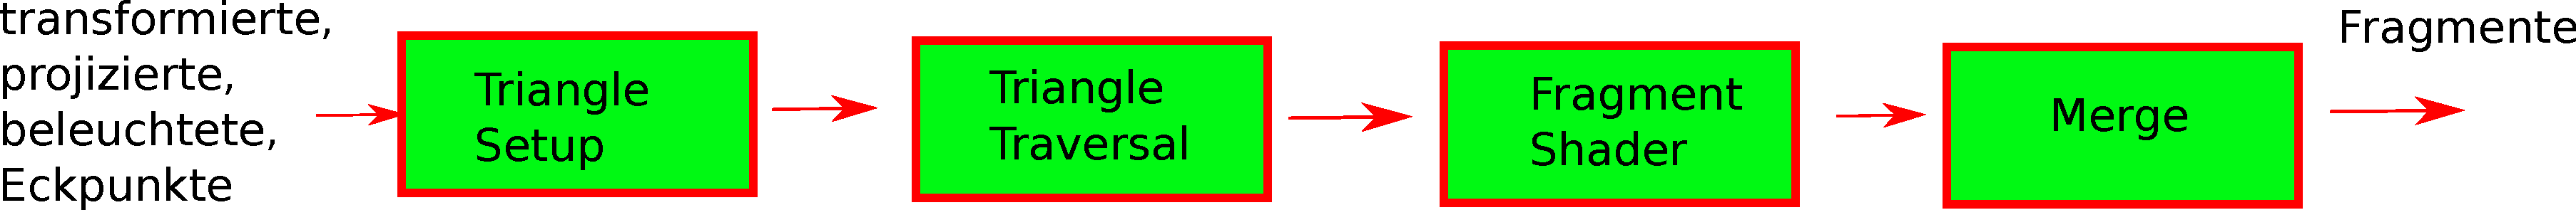
\includegraphics[width=\linewidth]{content/PathTracer/Bilder/Rasterisierung.pdf}
        \end{tcolorbox}
    \caption{Ablauf der Rasterisierung}
    \label{pic:Rasterisierungsablauf}
\end{figure}

        
Zuallererst befindet man sich im \nameref{pic:Rasterisierungsablauf} beim \textit{Triangle Setup}. Unbeeinflussbar vom Programmierer werden hier Daten berechnet, welche zur Pixeleinfärbung
benötigt werden. Beim darauffolgenden Schritt, dem \textit{Triangle Traversal}, werden die \textit{Fragmente} erzeugt, indem diejenigen Pixel bestimmt werden, welche innerhalb des Dreiecks liegen. 
Als freiprogrammierbare Shadereinheit können im \textit{Fragment Shader} vom Programmierer weitere Berechnungen vorgenommen werden. Dazu zählt eine pro Pixel Beleuchtungsberechnung (Phong Shading).
Das abschließende nicht komplett freiprogrammierbare, aber hoch konfigurierbare \textit{Merging} hat eine besondere Aufgabe beim Abspeichern der Farbe für
jeden Pixel im color Buffer. Zur Bestimmung der aktuellen Farbe wird nun auch das Problem der Sichtbarkeit von Objekten angegangen. Zu den Depth-Werten, welche wir als Tiefe beim 
Viewport Transform gespeichert haben, gibt es hier Zugang zum Depth-Buffer. Dieser Depth-Buffer speichert anfangs überall den Wert inf. Beim Durchlauf der Geometrie wird nun jeweils für jeden Pixel,
der die Geometrie bedeckt der color und depth buffer wie folgt aktualisiert: Ist der verglichene Tiefenwert des vom Objekt erzeugten Fragment kleiner als der Wert
im Tiefenbuffer für den betroffenen Pixel, so schreibt er diesen Tiefenwert in den Depth-Buffer und auch der color Buffer mit der Fragmentfarbe aktualisiert.
Falls nicht passiert nichts und das nächste Primitiv bzw. Fragment wird betrachtet. 
Eine Möglichkeit ist die Ausgabe, bestehend aus Lichter, Normalen, Tiefenwert, Farbe (sog. \textit{GBuffer}) in mehrere verschiedene \textit{render targets} zu schreiben. 
Wir werden zur Beschleunigung der globalen Beleuchtung durch einen \nameref{ch:Content1:sec:Path Tracer} einen solchen durch Rasterisierung berechneten \textit{GBuffer}(siehe auch
Abschnitt \ref{pic:Render Graph}) verwenden.
\par

\subsection{Beschränktheit}
\label{sec:Rasterisierung:Beschränktheit}

\begin{figure}[H]
    \begin{tcolorbox}
    \centering
    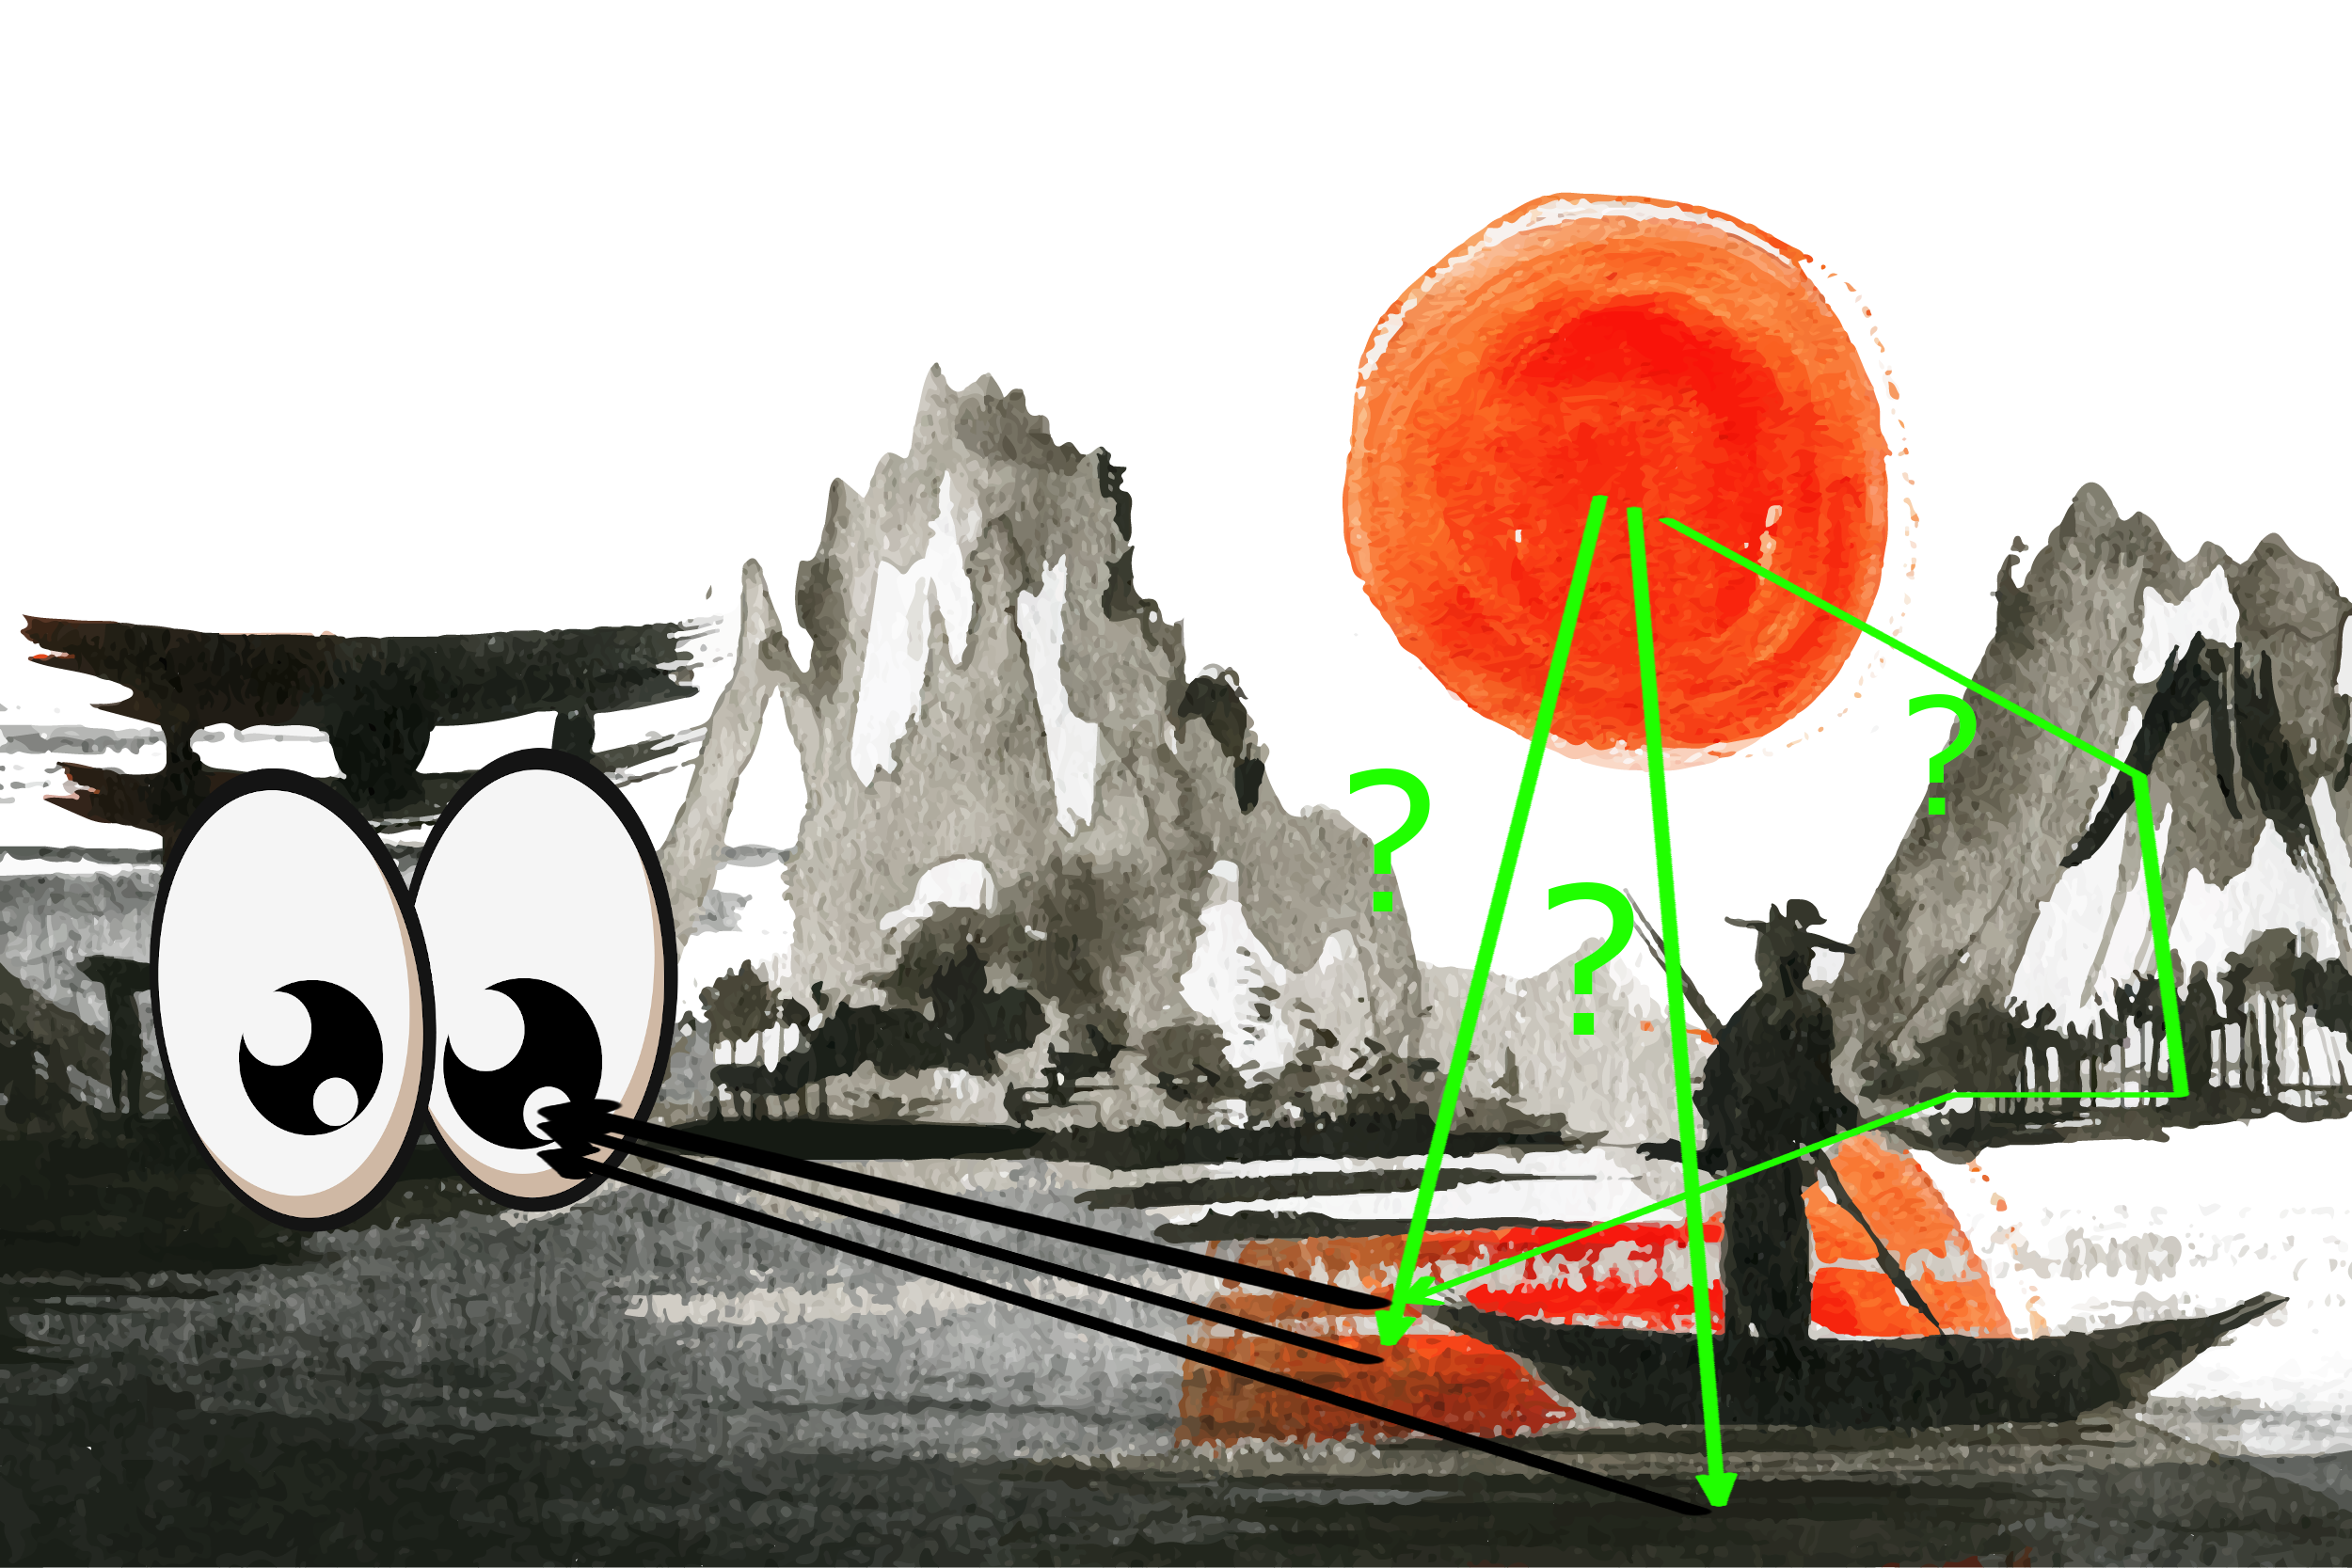
\includegraphics[width=\linewidth]{content/PathTracer/Bilder/RasterizerGuide.png}
    \end{tcolorbox}
    \caption{Ablauf der Rasterisierung}
    \label{pic:RasterizerGuide}
\end{figure}

Ihre bisherige weite Verbreitung hatte die Rasterisierung der Objektorientierung zu verdanken: massives paralleles Arbeiten, Ignorieren von (großen) leeren Bereichen und
Ausnutzen von Cachekohärenzen gehören zu den Eigenschaften, welche die enorme effiziente, schnelle Abarbeitung bzw. (relativ) geringe aufzuwendende Rechenleistung begründen.
Jedoch liegt in ihr auch die Crux.
Die Abbildung der Farbe eines Geometrie/Dreiecks auf einen Pixel simuliert
den physikalischen Lichttransport nicht korrekt! Die physikalische Optik lehrt uns das Verfolgen von weiteren (sekundären) Strahlen 
(siehe grüne Pfeile in Abbildung \ref{pic:RasterizerGuide})abseits des Primärstrahls, der von 
Sichtebene zum Objekt verläuft und durch die Rasterisierung im Gegensatz zu den Sekundärstrahlen abgedeckt wird. Abbildung \ref{pic:RasterizerGuide} verdeutlicht das 
Problem der Objektorientierung und deren Problem mit Sekundärstrahlen. So können Effekte, welche diese Sekundärstrahlen involvieren, 
entweder nicht oder nur (unzureichend befriedigend) dargestellt werden (Spiegelungen, Schatten und Pfade mit größerer Pfadlänge). \par

Die enormen Leistungsanforderungen von Technologien, welche diesen physikalisch korrekten Lichttransport möglich machen, haben sie bisher für Echtzeitanwendungen ausgeschlossen 
und führten zu nicht physikalisch korrekten Approximationstechnicken.
In heutigen modernen Grafikprogrammierschnittstellen (Vulkan, DirectX) jedoch befindet sich Raytracing-Funktionalität, welche auf Hardwareseite unterstützt wird.
Diese Unterstützung erlaubt neuerdings effizientere image-ordered Bilderstellungen in Echtzeit.  
Aktuelle Bemühungen gehen nun daran Strahlenerzeugung und Rasterisierung zu kombinieren. \cite{Barre-Brisebois2019} stellte
mit dem Spiel \textit{PICA PICA} eine solche Rendering-Pipeline vor, welche mithilfe von Path Tracing
(siehe Abschnitt \ref{ch:Content1:sec:Path Tracer}) arbeitet. Dabei wird der G-Buffer
(Texturen die Position, Normalen, Belichtung eines Bildes speichern) noch über Rasterisierung berechnet. Direkten Schatten kann man durch
rechengünstigere Approximationstechnicken oder durch das Verschießen von Strahlen bekommen. Diese Option verspricht eine Anpassungsfähigkeit der Pipeline nach Leistungsfähigkeit der Hardware. Ähnlich können nun
Reflexionen, Global Illumination, Ambient Occlusion und Transmission durch Verschießen von Strahlen oder auf Compute Shader ausgeführt werden (wieder je nach 
Hardwareleistung). Einzig direkte Beleuchtung sowie Post-Processing Effekte laufen nur über Compute-Shader. \par

Wir wollen diesen Ansatz in dieser Arbeit aufnehmen. Berechnung des \textit{GBuffer}'s mit Hilfe von Rasterisierung und globale Beleuchtung durch 
einen \nameref{ch:Content1:sec:Path Tracer} erreichen. Da trotz hardwarebeschleunigtes Strahlenverschießen unsere Anzahl an Strahlen beschränkt ist, 
beschäftigen wir uns innerhalb dieser Arbeit mit einem \nameref{ch:Temporaler Algorithmus}, der die visuelle Qualität nicht durch Verschießen von mehr Strahlen, 
sondern durch eine zeitlich stabile \nameref{ch:Content1:sec:blue noise} Fehlerverteilungen im Bildraum erreicht.
%% ===========================

%% ===========================
\newpage
\section{Path Tracer}
\label{ch:Content1:sec:Path Tracer}
\subsubsection{Funktionsweise}
In offline Produktionen bereits fest etabliert \cite{DisneyPathTracing} so gewinnt diese Technik
der Bilderzeugung durch neue Hardwareunterstützung für Echtzeitanwendungen an Aufmerksamkeit\cite{Sch19}.
Anstatt vom Objekt wird die Bilderzeugung ausgehend vom Betrachter angesetzt 
(siehe Abbildung\ref{pic::GrundkonzeptPathTracing}).
Bei der Bilderzeugung, ausgehend von Szenen, welche viel Geometrie beinhalten bzw. bei Szenen 
die generelle BRDF's verwenden eignet sich der \nameref{ch:Content1:sec:Path Tracer}.

\begin{figure}[H]
    \centering
    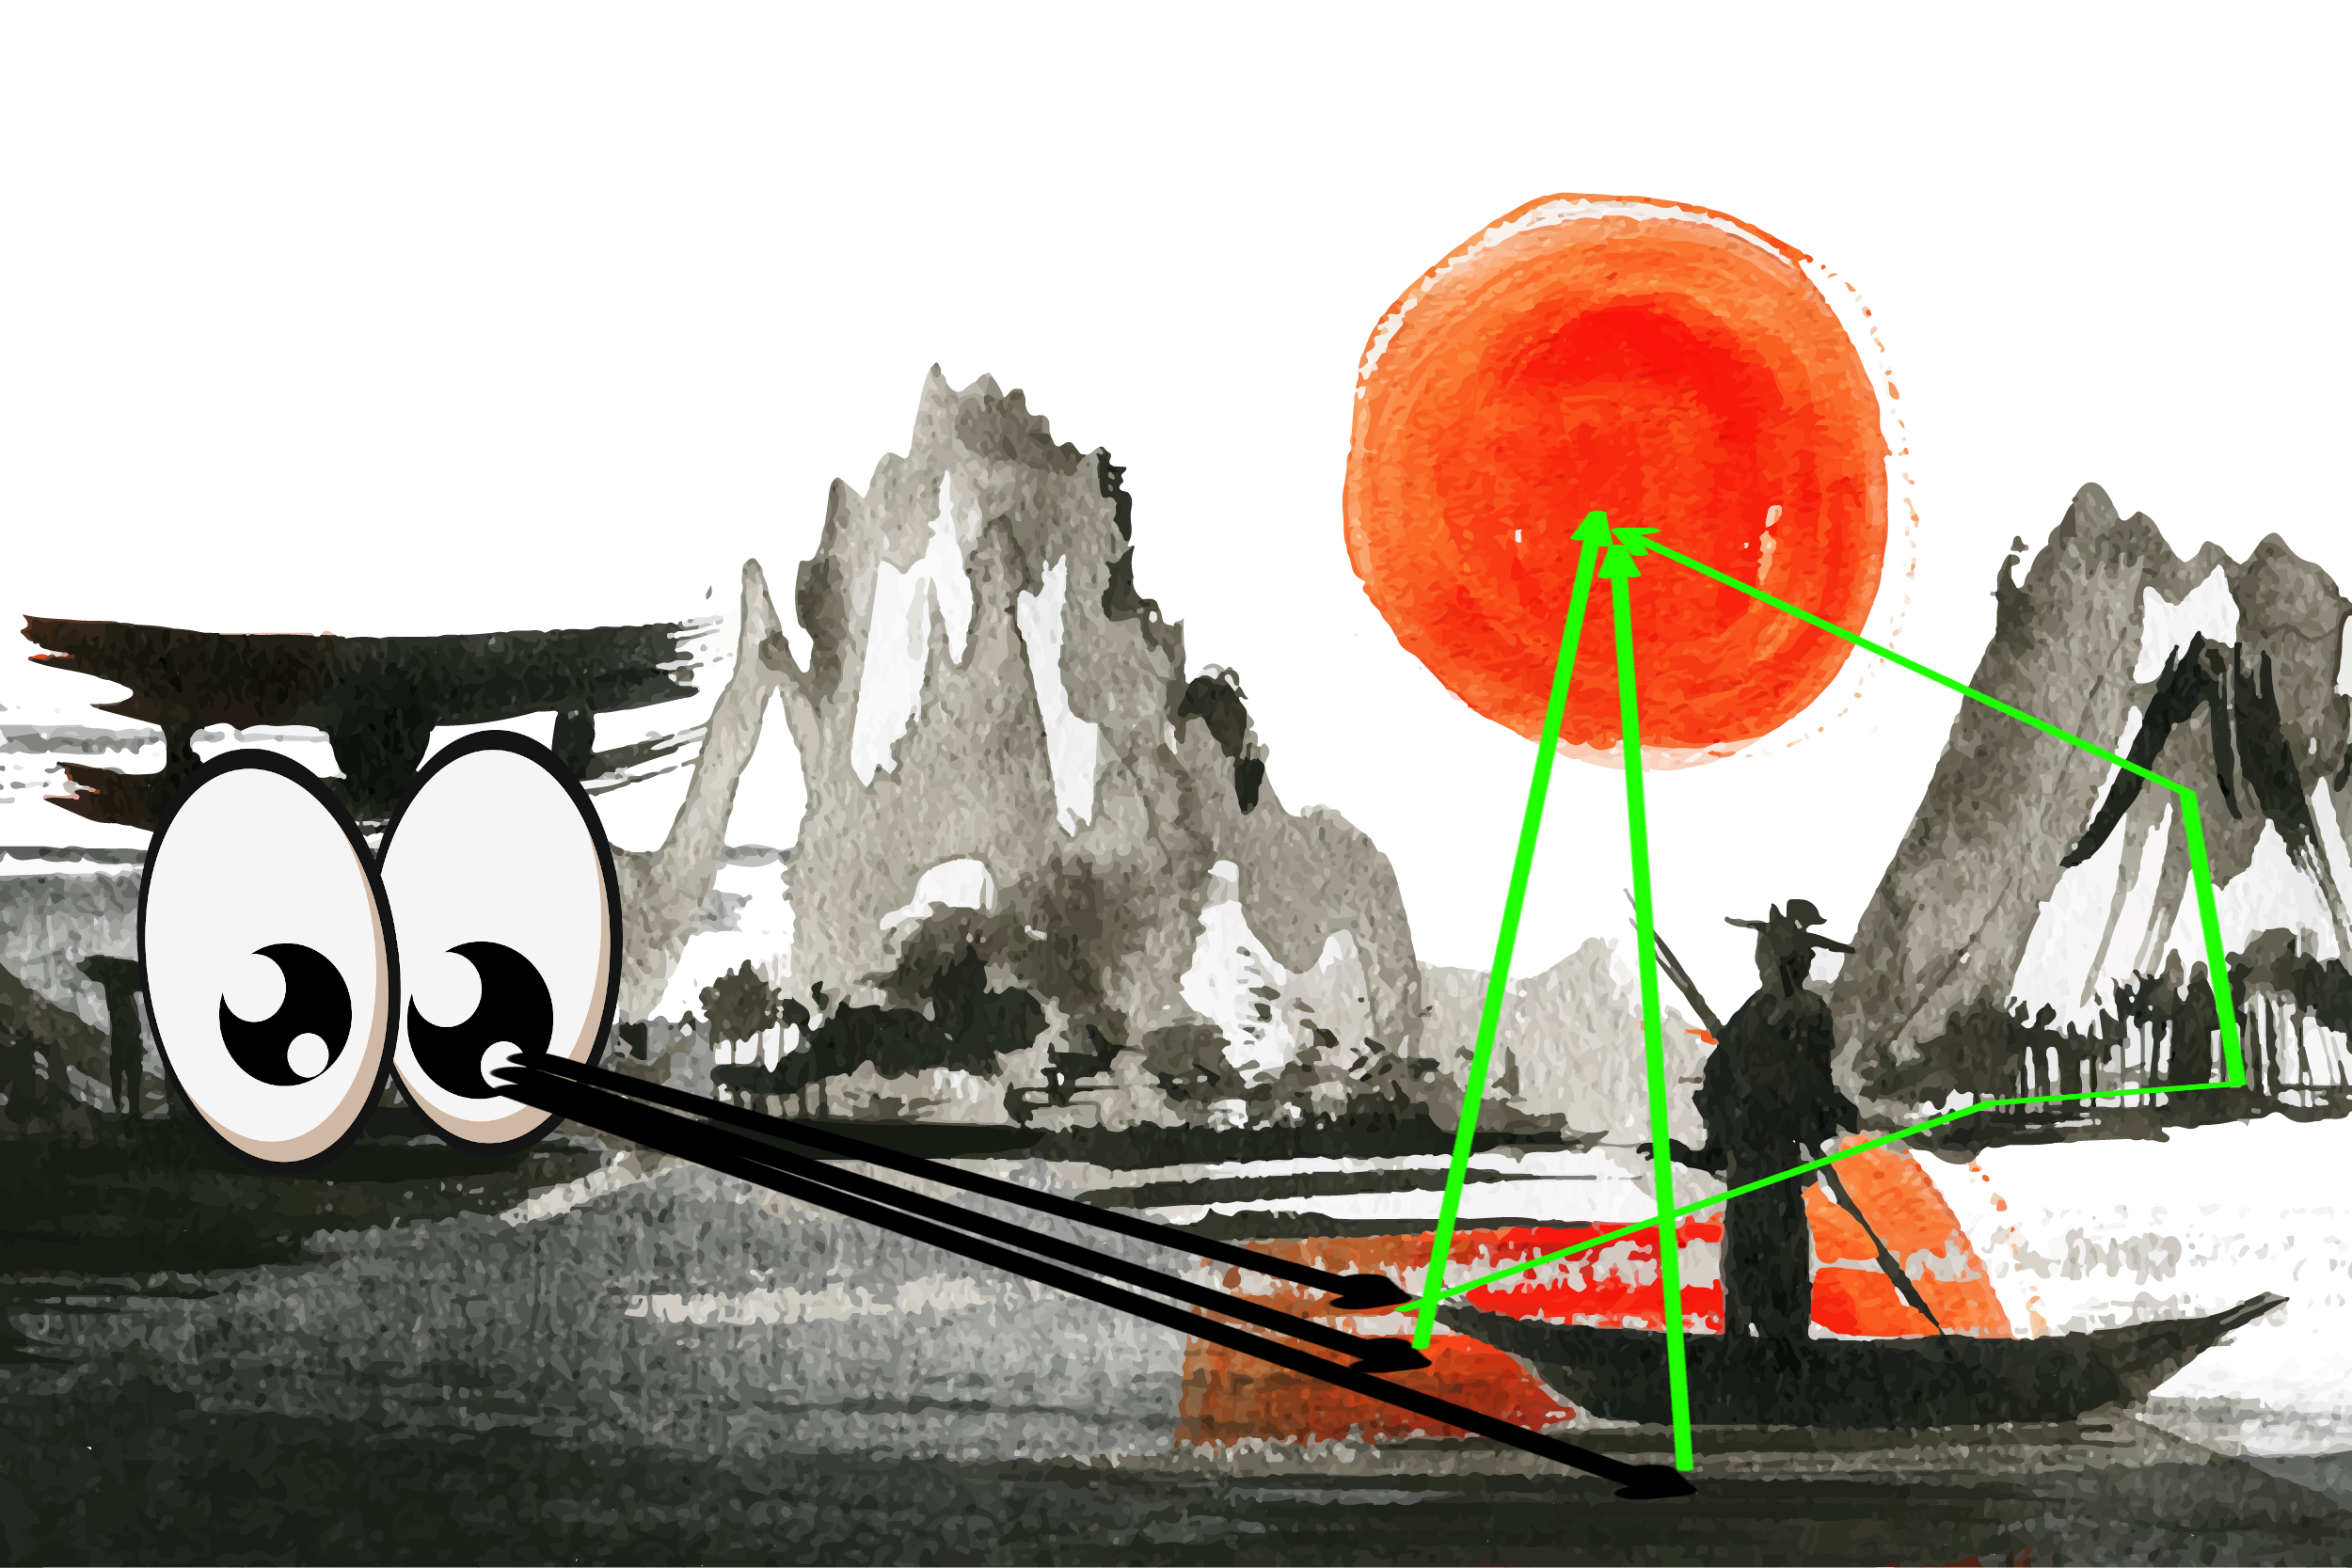
\includegraphics[width=\linewidth]{content/PathTracer/Bilder/PathTracerGuide.png}
    \caption{Grundkonzept Path Tracer}
    \label{pic::GrundkonzeptPathTracing}
\end{figure}

Der \nameref{ch:Content1:sec:Path Tracer} ist in Hinsicht der Beleuchtung komplett. Deshalb lässt sich damit
\textit{Global Illumination} erreichen. Der hier verwendete \nameref{ch:Content1:sec:Path Tracer} in 
\cite{Benty18} verwendet eine klassische Umsetzung.\par
Der Path Tracer beruht auf Erkenntnisse der Lösung der allgemeinen Rendergleichung.\nameref{eq:Allgemeine Rendergleichung}

\begin{equation}\label{eq:Allgemeine Rendergleichung}
    I(x,{x}^{'}) = g(x,{x}^{'}) * \biggl[\epsilon(x,{x}^{'}) + 
    \int_{S}^{} \rho(x,{x}^{'},{x}^{''})
    I({x}^{'},{x}^{''}d{x}^{''})\biggr] 
\end{equation}

Sie beschreibt den Energietransport \textit{I} von einem Punkt ${x}^{'}$
zu einem Punkt x. Dabei ist ein maßgebender Faktor der Geometrieterm \textit{g},
der die relative Lage der beiden Punkte zueinander im Raum beschreibt.
Ein weiterer Faktor ist die Abstrahlung \textit{$\epsilon$} von ${x}^{'}$ nach x. 
Beeinflusst wird der Energiefluss auch durch
die bidirektionale Verteilungsfunktion \textit{$\rho$}, welche Aufschluss über
das einfallende Licht von einem Punkt ${x}^{''}$ über ${x}^{'}$ zu x gibt.\par
Die Schlussfolgerung aus dieser Gleichung \nameref{eq:Allgemeine Rendergleichung} ist: Die transportierte
Intensität von einem Licht zu einem Anderen ist die Summe des ausgestrahlten Lichts 
und das ausgestrahlte Licht zu x von allen anderen Oberflächen.

Ausgehend von der Rendergleichung \nameref{eq:Allgemeine Rendergleichung} lässt sich
die vollständige Transportgleichung\nameref{eq:vollständige Transportgleichung} des \nameref{ch:Content1:sec:Path Tracer}
beschreiben.
Wie von \cite{marschner2009fundamentals} beschrieben wird ausgehend von der vollständigen Transportgleichung
\nameref{eq:vollständige Transportgleichung}

\begin{equation}\label{eq:vollständige Transportgleichung}
    L_s(k_0) = L_e(k_0) + \int_{all(k_i)}^{} \rho(k_i, k_0)*L_f(k_i)*cos(\theta_i)d\theta_i
\end{equation}

der vollständige Lichttransport beschrieben. Man kann deutlich die Ähnlichkeit
zu \nameref{eq:Allgemeine Rendergleichung} erkennen. Wir haben den Emissionsterm, die relative Lage der 
Punkte zueinander und die bidirektionale Verteilungsfunktion welche den Energietransport
beeinflussen.


\subsubsection{Monte-Carlo-Integration}
Mit der Monte Carlo Integration approximieren wir die Rendergleichung.\par 
Bei gegebener Dimensionalität n des Renderintegrals und der 
Wahrscheinlichkeitsdichtefunktion $\rho(x_i)$
\cite{KK02}

\begin{equation}\label{eq:Monte-Carlo}
    E\biggl[\frac{1}{k}\sum_{i=1}^{k}\frac{f(X_{i}}{\rho(X_{i})})\biggl] = \int_{[0,1]^{n}}f(x)dx
\end{equation}

Dabei wird das n-dimensionale Integral\nameref{eq:vollständige Transportgleichung} approximiert. Die Dichtefunktion $\rho(x_i)$ 
beschreibt deutet an, dass hierbei die Stichproben auch nicht-uniform 
genommen werden können. Varianzreduktionsmethoden machen sich diese Dichtefunktion zu Nutze um 
ein besseres Ergebnis zu bekommen.
\cite{caflisch_1998}
Konvergenzrate, unabhängig von der Dimension unseres Tracers.\textit{O}($N^{-\frac{1}{2}}$).
Sie ist robust, das heißt Exaktheit hängt nur vom ungenauesten Parameter ab. Eine Variante des Verfahrens, 
Monte Carlo Quadratur, wird mit quasi zufälligen Sequenzen \nameref{ch:Content1:sec:Quasi-Zufallsfolgen}, 
welche eine niedrige Abweichung aufweisen, durchgeführt. Laufzeit quasi-Monte Carlo \textit{O}(($\log N)^{k}N^{-1}$).
Um die Konvergenzrate zu steigern liegen eine Reihe von Varianzreduktionsmethoden vor.

Abseits dieser herkömmlichen Strategien zeigen wir hier die Steigerung der 
visuellen Qualität durch blue noise Fehlerverteilung im Bildraum.

\begin{equation}\label{eq:Monte-Carlo-Varianz}
    V[X] = E\biggl[(X-E[X])^{2}\biggl] = E[X^{2}]
    - E[X]^{2}
\end{equation}

Die Varianz \nameref{eq:Monte-Carlo-Varianz} ist ein quadratischer Fehler.

\subsubsection{DirectX Raytracing}

\begin{figure}[H]
    \centering
    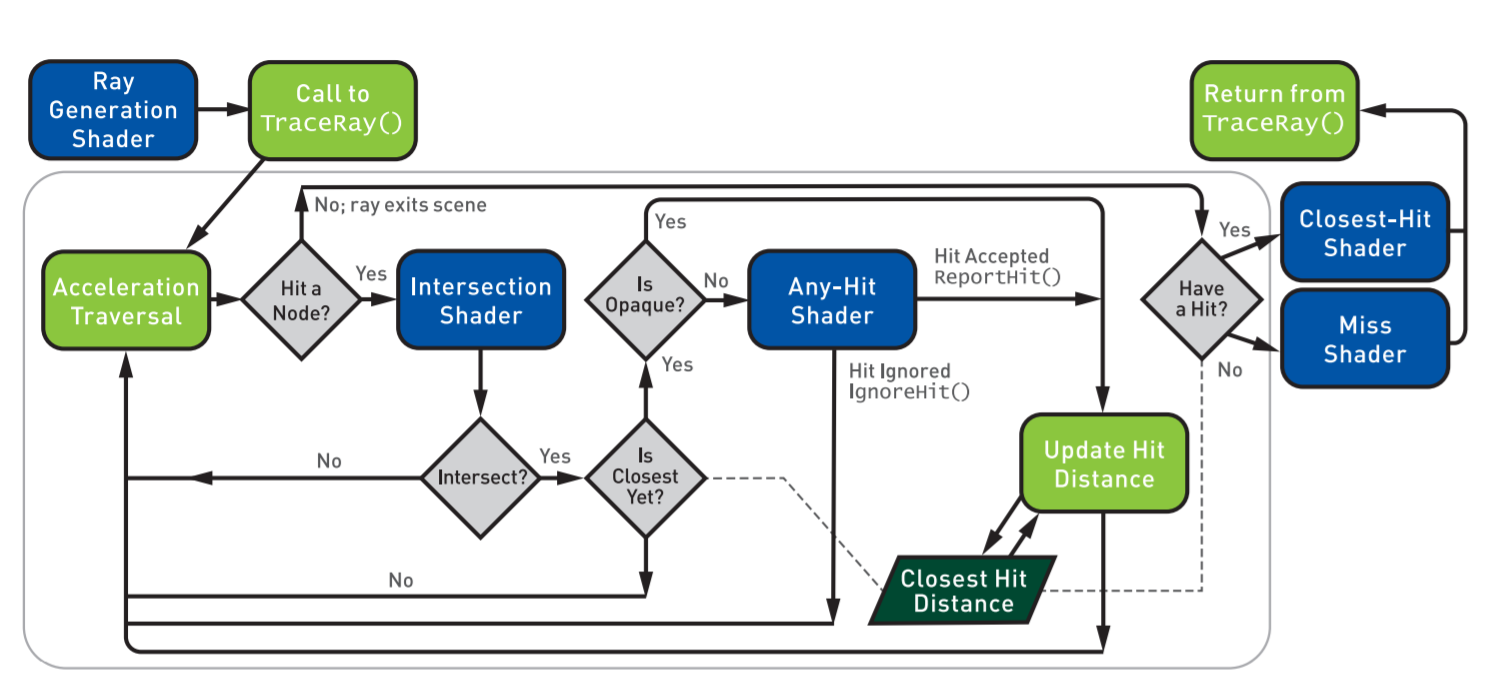
\includegraphics[width=\linewidth]{content/PathTracer/Bilder/DirectXRaytracingPipeline.png}
    \caption{DirectX Raytracing Pipeline aus \cite{Haines2019}}
    \label{pic:DirectXRaytracingPipeline}
\end{figure}

In \ref{pic:DirectXRaytracingPipeline} lässt sich der Beginn (Generierung eines Strahles) der neuen Pipeline
durch den programmierbaren \textbf{Ray Generation shader} erkennen.

\begin{algorithm}[H]
    \caption{Beispielhafter minimalistischer Ray Generation Shader}
    \begin{algorithmic}[1]
        \State [shader(\dq raygeneration \dq)]
        \State launchIndex = DispatchRaysIndex().xy;
        \For{(int i = 0; i < numberOfRays;i++)}
            \State float shadowRayMult = TraceRay(gRtScene,
            RAY\_FLAG\_ACCEPT\_FIRST\_HIT \_AND\_END\_SEARCH |
            RAY\_FLAG\_SKIP\_CLOSEST\_HIT\_SHADER,
            0xFF, 0, hitProgramCount, 0, ray, payload);
            \State float indirectRayColor = TraceRay(gRtScene, 0, 0xFF, 1, hitProgramCount, 1, rayColor, payload);
            \State color = shadowRayMult * shadingColor + computeindirectLighting(indirectRayColor);
        \EndFor
        \State output[id] = color;
    \end{algorithmic}
    \label{alg:Ray Gen}
\end{algorithm}

Mit Hilfe der Methode \textbf{TraceRay()} werden dann zur Beleuchtungsberechnung 
die Strahlen verschossen. Damit diese Methode richtig arbeiten kann übergeben wir neben unseren Strahl 
unter Anderem  unsere Szene inklusive Beschleunigungsstruktur, rayflags 
(beeinflussen Transparaenz, Culling, Abbruch)\cite{RayFlags} und einen payload.
Mit dem \textit{$payload_t$} Typ können wir einen struct mit Informationen jedem einzelnen Strahl mitgeben.

\begin{algorithm}[H]
    \caption{beispielhafter payload}
    \begin{algorithmic}[1]
        \State struct RayPayload = {
            \State        float4 color, uint32 seed, uint32 depth
            \State };
        \end{algorithmic}
        \label{alg:payload}
    \end{algorithm}
    
Diese Methode \textbf{TraceRay()} kann auch innerhalb der anderen Shader zum weiteren verschießen
von Strahlen verwendet werden. Beispiel beim Verschiessen vom Schattenstrahl: Flags 
RAY\_FLAG\_ACCEPT\_FIRST\_HIT\_AND\_END\_SEARCH, \newline
RAY\_FLAG\_SKIP\_CLOSEST\_HIT\_SHADER setzen, um unnötige 
Shadingberechnungen und weitere Schnittpunktberechnungen zu umgehen und mit einem Bit als payload 
die Sichtbarkeit zur Lichtquelle mitgeben.


Mit diesem beispielhaften payload können wir die Farbe akkumulieren, unseren verwendeten 
seed verwenden um z.B eine weiteren Strahlenschuss in einem Any-Hit Shader zu verwirklichen,  
solange die mit übergebene Rekursionstiefe in unserem payload eingehalten wird.  

\textbf{Intersection shader} führt die Schnittberechnungen durch.
Haben wir eine Szene, welche aus ausschließlich Dreiecken besteht, können wir
die auf Hardware standardmäßig gelieferte Implementierung übernehmen. 
Optionale Berechnungen für andere Geometrie können hier implementiert werden.
Bei einem gefundenen nähsten Schnittpunkt einer durchsichtigen Oberfläche wird der 
\textit{Any-hit shader} aufgerufen.
\textbf{Any-hit shaders} erlauben klassische \textit{Discards} oder informieren
über einen korrekten Schnitt. So können wir z.B. einen Alpha Test durchführen.

\begin{algorithm}[H]
    \caption{Any-Hit shader}
    \begin{algorithmic}[1]
        \State [shader(\dq anyhit \dq)]
        \If{(!alphaTest)} 
        \State IgnoreHit();
        \EndIf
    \end{algorithmic}
    \label{alg:any hit}
\end{algorithm}

Der \textbf{Closest-hit shader} berechnet den Schnittpunkt des Strahls mit der Geometrie
der Szene, die dem Strahlursprung am nähesten ist.
Mit der Kennzeichnung [shader(\dq closesthit \dq)] wird die Hauptmethode zur 
dessen Ausführung markiert. An dieser Stelle bietet es sich an die Shading Farbe 
mit der Schnittpunktinformation zu aktualisieren und/oder um eine Rekursionstiefe weiter 
zu gehen einen weiteren Strahl zu verschießen. 
Der \textbf{miss shader} wird immer dann ausgeführt, wenn ein Strahl die
Szenengeometrie nicht schneidet. Kann also für das Nachschauen in einer 
Environment Map verwendet werden. Im Folgenden \nameref{alg:Path Tracer Konzept}
nochmal vereinfacht in Pseudocode dargestellt, wobei die entsprechenden shader
im jeweiligen Codeabschnitt markiert sind.

\begin{algorithm}[H]
    \caption{Path Tracing Algorithmus}
    \begin{algorithmic}[1]
        \Procedure{Trace Path}{$BVH$}\Comment{verfolge Pfad durch Szene}
        \For{(x,y) $\in$ frame}
        \State strahl = verschiesseStrahlInPixel(x,y); // \textbf{ray generation shader}
        \For{blatt = bekommeBVHBlatt()}
        \State schnittpunkt = schneideGeometrie(strahl, blatt); //\textbf{Intersection shader}
        \If{schnittpunkt $\leq$ nähesterSchnittpunkt}
        \State aktualisiereNähestenSchnittpunkt();
        \EndIf
        \EndFor
        \If{Schnittpunkt gefunden}
        \State frame(x,y) = gebeFarbe(strahl,nähesterSchnittpunkt); //\textbf{closest-hit shader}
        \Else
        \State frame(x,y) = Umgebungskarte(x,y);//\textbf{miss shader}
        \EndIf
        \EndFor
        \EndProcedure
    \end{algorithmic}
    \label{alg:Path Tracer Konzept}
\end{algorithm}

\subsection{RenderGraph}

\begin{figure}[H]
    \centering
    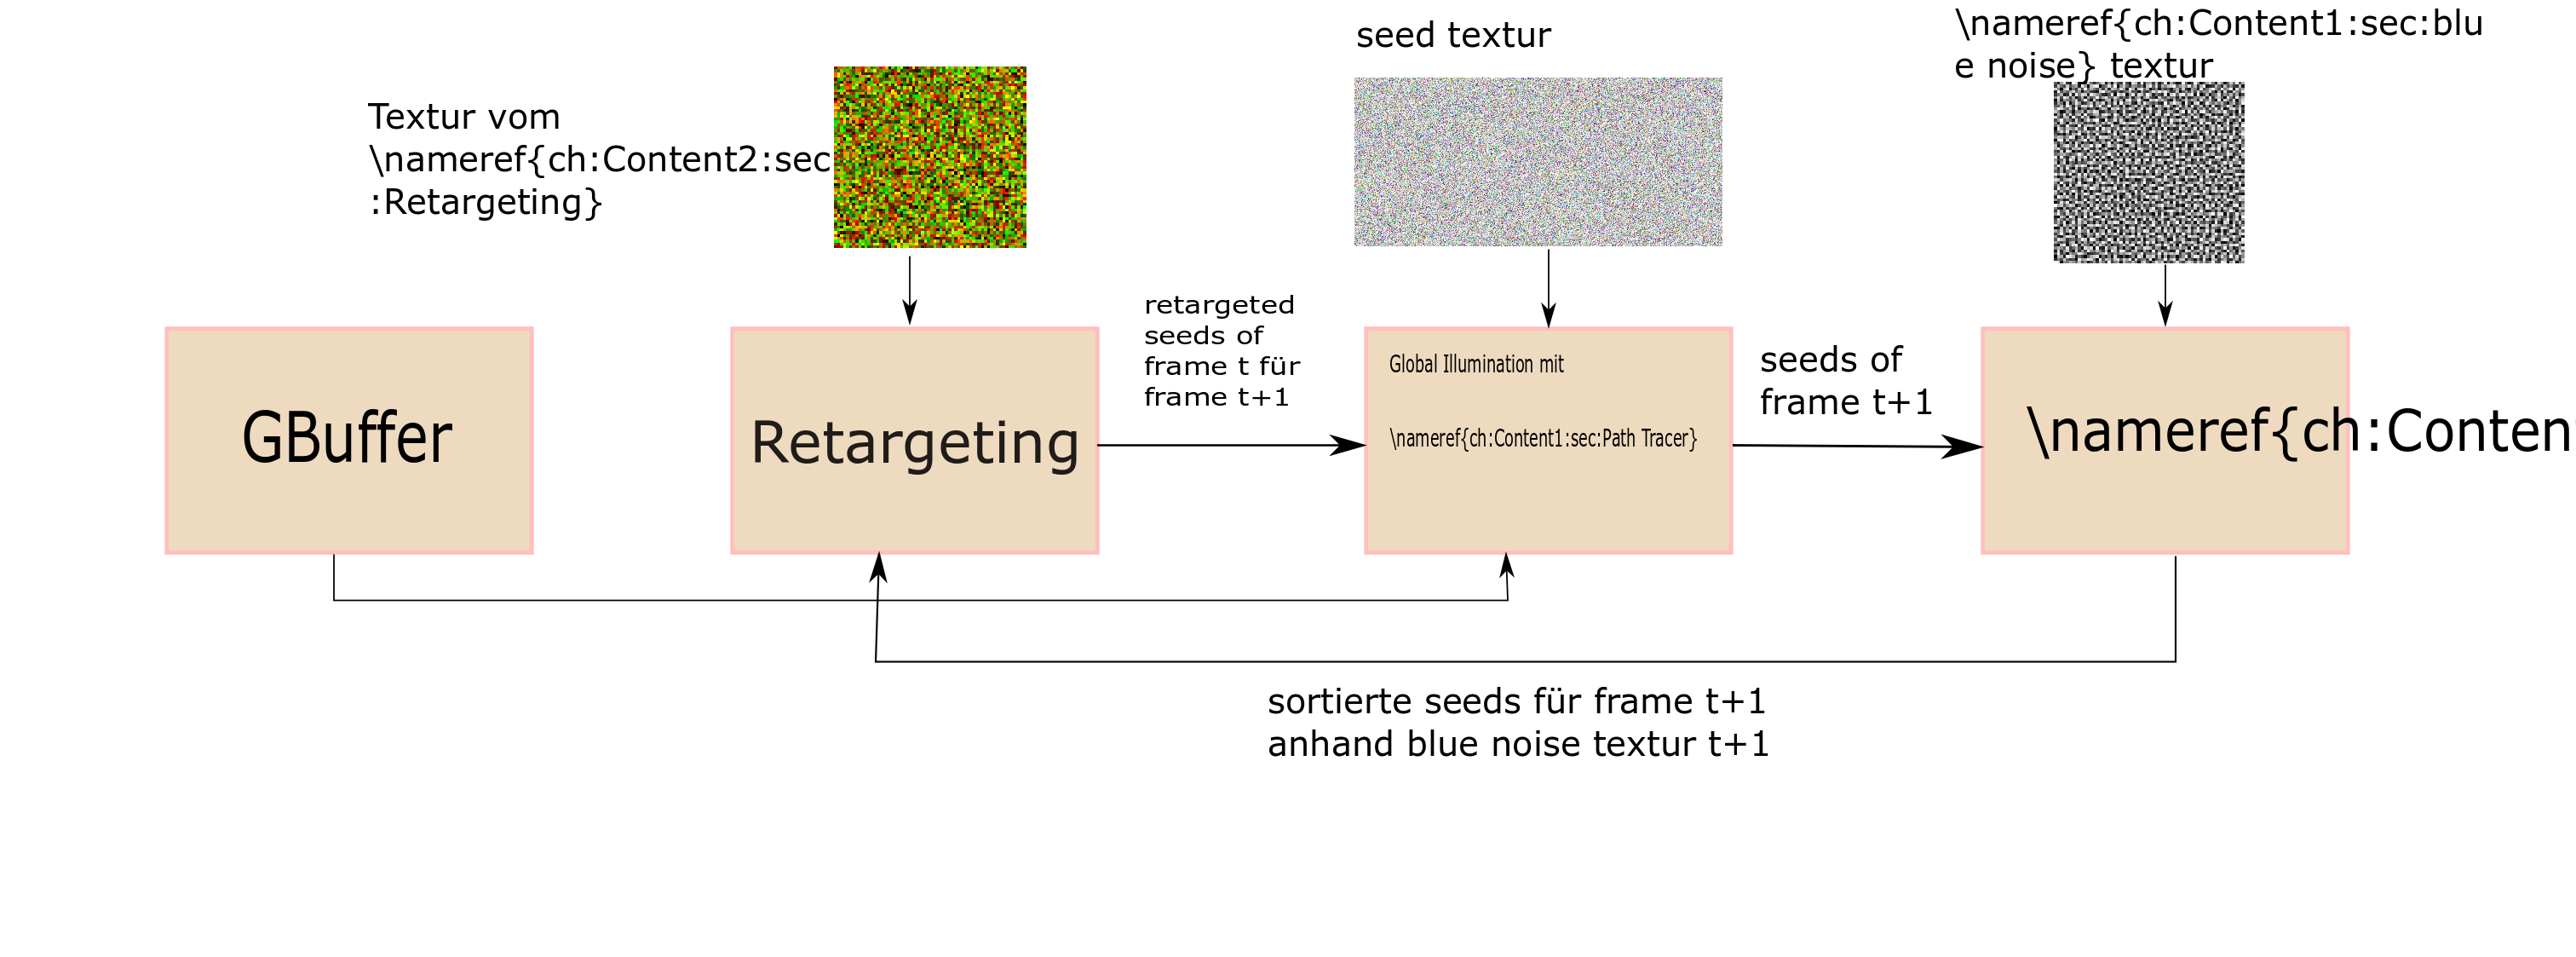
\includegraphics[width=\linewidth]{content/PathTracer/Bilder/render_graph.png}
    \caption{Unser Render Graph}
    \label{pic::RenderGraph}
\end{figure}





%% ===========================


%% ===========================
\newpage
\section{Blue Noise}
\label{ch:Content1:sec:blue noise}
\subsection{Eigenschaften}

Wie in \cite{Pet17} vorgestellt, macht man sich die Eigenschaften einer
blue noise Textur zu Nutze. Dabei werden im Folgenden, die dort bereit 
gestellten blue noise verteilten Texturen verwendet, welche anhand des in
\cite{ulichney1993void} vorgestellten Algorithmus erstellt wurden.
Die korrespondierenden Spektren werden mit Hilfe von \cite{FFTProgWeb} erstellt.

\subsubsection{Uniformität}
Die Uniformität(lat. \textit{uniformitas}-Einförmigkeit) garantiert uns 
wie in \cite{3288} eine gleichverteilte Wahrscheinlichkeitsdichtefunktion
mit zugehöriger gleichverteilter Wahrscheinlichkeitsfunktion. In \cite{Pet17}
sieht sie wie folgt aus: 

\begin{equation}\label{eq:uniformität}
    P(n \leq p) = p
\end{equation}

\cite{kiencke2009signale}

\subsubsection{Niedrige Frequenzen}
Niedrige Frequenzen sind in einer blue noise sehr wenig bis gar nicht 
vertreten. Dies ist an dem schwarzen Ring innerhalb der Fouriertransformierten
zu erkennen\ref{pic:blueNoiseFFT}.

\begin{figure}[H]\label{pic:blueNoiseFFT}
    \centering
    \begin{minipage}[t]{0.45\linewidth}
        \centering
        
\includegraphics[width=\linewidth]{content/BlueNoise/Bilder/LDR_LLL1_0.png}
        \caption{$512^{2}$ blue noise Textur}
    \end{minipage}
    \hfill
    \begin{minipage}[t]{0.45\linewidth}
        \centering
        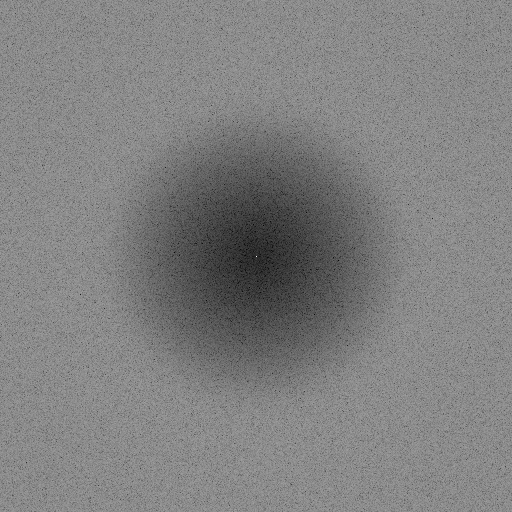
\includegraphics[width=\linewidth]{content/BlueNoise/Bilder/FFT_LDR_LLL1_0.png}
        \caption{Fourier Spektrum $512^{2}$ blue noise Textur}
    \end{minipage}
\end{figure}

\begin{figure}[H]\label{pic:bayerPatternFFT}
    \centering
    \begin{minipage}[t]{0.45\linewidth}
        \centering
        
\includegraphics[width=\linewidth]{content/BlueNoise/Bilder/BayerMatrix.png}
        \caption{$512^{2}$ bayer pattern Textur}
    \end{minipage}
    \hfill
    \begin{minipage}[t]{0.45\linewidth}
        \centering
        
\includegraphics[width=\linewidth]{content/BlueNoise/Bilder/FFT_BayerMatrix.png}
        \caption{Fourier Spektrum $512^{2}$ bayer pattern Textur}
    \end{minipage}
\end{figure}

\begin{figure}[H]\label{pic:tiledBlueNoiseFFT}
    \centering
    \begin{minipage}[t]{0.45\linewidth}
        \centering
        
\includegraphics[width=\linewidth]{content/BlueNoise/Bilder/BlueNoise64Tiled.png}
        \caption{$512^{2}$ bayer pattern Textur}
    \end{minipage}
    \hfill
    \begin{minipage}[t]{0.45\linewidth}
        \centering
        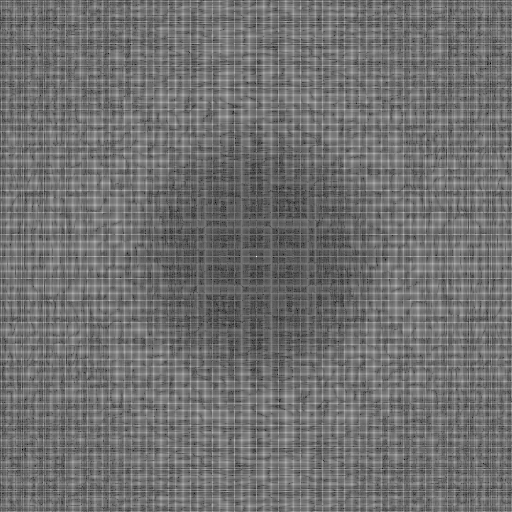
\includegraphics[width=\linewidth]{content/BlueNoise/Bilder/FFT_BlueNoise64Tiled.png}
        \caption{Fourier Spektrum $512^{2}$ bayer pattern Textur}
    \end{minipage}
\end{figure}

\subsubsection{Isotropie}
Die Isotropie(altgr. \textit{isos}-gleich und \textit{tropos}-Richtung)
einer blue noise Textur wird ausgenutzt. Dabei haben wir in allen
Dimensionen (in dieser Arbeit werden Texturen mit zwei benutzt) 
die Unabhängigkeit einer Eigenschaft. 


\subsubsection{Kachelung}
Eine weitere nützliche Eigenschaft der blue noise Verteilung ist die 
Möglichkeit der Kachelung. 
%% ===========================


%% ===========================
\newpage
\section{Quasi-Zufallsfolgen}
\label{ch:Content1:sec:Quasi-Zufallsfolgen}
\cite{owen1998scrambling} \cite{heitz:hal02150657}


\subsection{Einleitung}
Quasi-zufällige Sequenzen mit niedriger Abweichung sind deterministisch 
erzeugte Sequenzen, welche die Likelihood-Funktion der Clusterbildung

\begin{equation}\label{eq:Likeli-Hood-Gleichung}
    L_{x}(\delta) = f_{\delta}(x)
\end{equation}

minimieren. Dabei behalten wir die Eigenschaft einer zufälligen Folge, 
den gesamten Platz gleichmäßig auszufüllen. Diese Eigenschaften erinnern
uns an die besprochenen Eigenschaften bei \nameref{ch:Content1:sec:BlueNoise}.
Im Folgenden wird für uns der zweidimensionale Fall wichtig sein, weswegen
wir vom ein- über zum zweidimensionalen schauen werden.

\label{subsec:onedimensional}
\subsection{1-Dimension}
Diese Arbeit betrachtet Rekurrenz Sequenzen, basierend auf irrationalem 
Bruchrechnen der Form
\begin{equation}\label{eq:Rekurrenz Sequenz}
    R_{1}(\alpha) : t_n = s_0 + n\alpha(mod 1); n = 1,2,3,...
\end{equation}
wobei $\alpha \in \mathbb{I}$ und das (mod 1) einen \textit{"toroidally shift"}
bezeichnet. Will man mit dieser Formel eine Sequenz mit möglichst geringer
Abweichung schaffen, und genau das wollen wir, so wählen wir 
$\alpha = \Phi$ wobei $\Phi \approx 1.618033$ den goldenen Schnitt bezeichnet.
Wie \cite{quasirandomsequencesbyRoberts} gezeigt wird, ist diese Form von 
Sequenz die beste für das \nameref{eq:Rekurrenz Sequenz}.  

\subsection{2-Dimensionen}

Für mehrere Dimensionen, hier zwei, kombiniert man in gängigen Methoden 
einfach zwei \nameref{subsec:onedimensional} eindimensionale Sequenzen.
Für unsere Zwecke untersuchen wir hier die Generalisierung des bereits 
zuvor beschriebenen goldenen Schnitts \nameref{subsec:onedimensional}, wie
hier \cite{krcadinac2006new} beschrieben. 
Die sogenannte Plastische Zahl in ist die Lösung der
Gleichung \nameref{eq:plastische Nummer}
\begin{equation}\label{eq:kubisch}
   x^{3} - x - 1 = 0
\end{equation}
Die Lösung dieser Gleichung lässt sich über die Padovan und Perrin Sequenz
definieren. Damit erhalten wir Plastische Zahl $\Phi$:

\begin{equation} \label{eq:plastische Nummer}
   \Phi = \frac{(9 - \sqrt{69})^{1/3} + (9 + \sqrt{69})^{1/3}}
               {2^{1/3}3^{2/3}} \approx 1.32471795
\end{equation}

\cite{vanderlaanplasticnumber}
\cite{wolframalphaPlastic}
Folgende Gleichung ist auch einfach erweiterbar für höhere Dimensionen.
\begin{equation}\label{eq:1 zu N - Dimensional}
    t_{n} = n\alpha(mod 1), n = 1,2,3,..
    \alpha = (\frac{1}{\Phi_{d}}, \frac{1}{\Phi_{d}^{2}}),
\end{equation}
Dabei ist $\Phi_{d}$ der goldene Schnitt. $\Phi_{d}^{2}$ ist Lösung der
\nameref{eq:kubisch} obigen Gleichung.


\cite{quasirandomsequencesbyRoberts}
\begin{lstlisting}[style=CStyle]
   float g = 1.32471795724474602596; //Plastische Zahl
   float a1 = 1.0/g;
   float a2 = 1.0/(g*g);
   x[n] = (0.5+a1*n) %1; //toroidally shifted
   y[n] = (0.5+a2*n) %1; //toroidally shifted
\end{lstlisting}


\subsection{Dither Texturen und quasi-zufällige Folgen}

%% ===========================


%% ===========================
\newpage
\section{Simulated Annealing}
\label{ch:Content2:sec:Simulated Annealing}
Für unseren temporalen Algorithmus (siehe Abschnitt \ref{ch:Temporaler Algorithmus}) gibt es einen 
wichtigen \nameref{ch:Content2:sec:Retargeting} Schritt.
In diesem Schritt wird eine vorberechnete Textur verwendet. Diese speichert eine
Permutation, die unsere \nameref{ch:Content1:sec:blue noise} Textur vom Bild t in eine
blue noise Textur von Bild t+1 umwandelt. Diese Permutation wird 
dann auf die Startwerte angewandt bevor das nächste Bild t+1 gerendert wird (siehe auch Übersicht \nameref{pic:Render Graph}).
Dadurch werden die blue noise Umverteilungen der \nameref{ch:Content2:sec:Sorting} Phase akkumuliert. 
All diese Vorberechnungen sind möglich, da wir mit \textit{\glqq nur\grqq} quasi-zufälligen Sequenzen 
(siehe Abschnitt \ref{ch:Content1:sec:Quasi-Zufallsfolgen}) arbeiten.
Das andauernde Permutieren von Pixeln bis zu einem Punkt, an dem ein Bild aussieht wie das Andere ist 
ein klassisches TSP, wofür es aktuell keine effiziente optimale Lösungsmethode gibt.
Da wir nur an einer sehr guten Lösung, nahe dem globalen Optimum, interessiert sind 
greifen wir wie in \cite{hal02158423} vorgeschlagen auf das heuristische Approximationsverfahren,
dem Simulated Annealing, zu.

\subsubsection{Allgemein}

Angelehnt an metallurgischem Aufheizen und dem sich anschließenden Abkühlen wollen wir eine approximativ
optimale Lösung finden. Wir haben also eine zu Anfang hohe Temperatur, welche durch eine Abkühlfunktionen
(siehe Abschnitt \ref{subsec:Abkühlfunktion} für Weiteres) verringert wird.
Wir definieren die Energie als pixelweisen Unterschied der sich in Abkühlung 
befindlichen bereits permutierten Textur und der $Textur_{t+1}$(siehe Abbildung \ref{eq:pixel energy function}). 
$Textur_{t+1}$ ist durch quasi Zufall (siehe Abschnitt \ref{ch:Content1:sec:Quasi-Zufallsfolgen}) bereits bekannt.
Mit Erkenntnissen aus\cite{georgiev2016blue} ergibt sich

\begin{figure}[H]
    \begin{tcolorbox}[rightrule=3mm, rounded corners=east]
    \[ E(SA) = \sum_{p \neq q}E(p,q) = \sum_{\forall i \in [0,N-1]} \Vert{p_{i}-q_{i}}\Vert \]
    \end{tcolorbox}
    \caption{\nameref{ch:Content1:sec:blue noise} Textur mit Dimension N; Pixel p von abkühlende 
    $Textur_{t=0}$; Pixel q von $Textur_{t=1}$}
    \label{eq:pixel energy function}
\end{figure}

Mit dem definierten Ziel, die Energiefunktion \ref{eq:pixel energy function} zu minimieren, wenden 
wir in jedem Schritt eine Permutation an und entscheiden anhand einer Akzeptanzwahrscheinlichkeitsfunktion
\ref{eq:Akzeptanzwahrscheinlichkeitsfunktion}, ob wir diese Permutation beibehalten.
Da wir in jedem Schritt nur eine Permutation anwenden, vereinfacht sich unsere Energiefunktion
\ref{eq:pixel energy function} zu 

\newpage

\begin{figure}[H]
    \begin{tcolorbox}[rightrule=3mm, rounded corners=east]
    \[ E(SA) = E(s_{previous}) + \Vert{p_{i}-q_{i}}\Vert + \Vert{p_{i 
        + permutation}-q_{i + permutation}}\Vert\]
    \end{tcolorbox}
  \caption{Zustand $s_{previous}$ ohne angewandte Permutation}
  \label{eq:vereinfachte pixel energy function}
\end{figure}


\begin{figure}[H]
    \centering
    \begin{subfigure}[b]{0.4\textwidth}
        \begin{tcolorbox}[rightrule=3mm, rounded corners=east]
            \begin{equation}\label{eq:Akzeptanzwahrscheinlichkeitsfunktion}
                P = e^{-(\Delta_{energy})/ temperature}
            \end{equation}
        \end{tcolorbox}
        \caption{Akzeptanzwahrscheinlichkeitsfunktion; Abhängig von Energie und aktueller Temperatur}
    \end{subfigure}
    ~ %add desired spacing between images, e. g. ~, \quad, \qquad, \hfill etc. 
      %(or a blank line to force the subfigure onto a new line)
    \begin{subfigure}[b]{0.7\textwidth}
        \centering 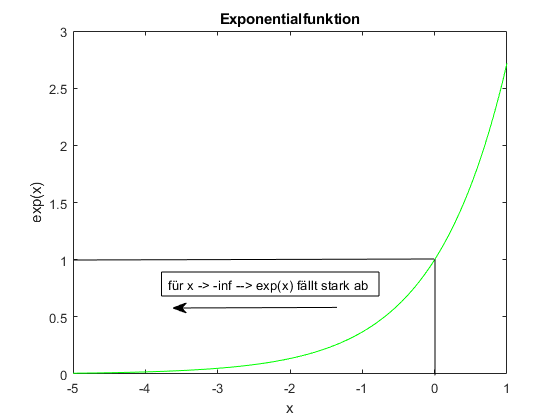
\includegraphics[interpolate=false,width=\linewidth]{content/simulatedAnnealing/Bilder/exponentialfunktion_as_PDF.png}
        \caption{Günstige Eigenschaft der Exponentialfunktion}
        \label{fig:Exponentialfunktion}
    \end{subfigure}
    \caption{}
\end{figure}

Die günstigen Eigenschaften der Exponentialfunktion (siehe Abbildung \ref{fig:Exponentialfunktion}) als
Wahrscheinlichkeitsakzeptanzfunktion sind vielfältig und bereits in weiterführender Literatur wie 
\cite{Kirkpatrick671},\cite{van1987simulated} gut belegt. Eine der Eigenschaften ist in der obigen Abbildung 
\ref{fig:Exponentialfunktion} dargestellt. Das Argument der Funktion \ref{fig:Exponentialfunktion} hat 
einen Divisor Temperatur und einen Dividenten $\Delta_{energie}$.
Mit absteigender Temperatur erkennt man 
in der Abbildung \ref{fig:Exponentialfunktion} eine ebenfalls abnehmende Wahrscheinlichkeit
der Akzeptanz. Dies führt zu dem gewünschten Verhalten, energiehöhere Zustände 
zuzulassen, um somit lokale Maxima zu verlassen. Dies geschieht bei höheren 
Temperaturen häufiger wohingegen bei niederen Temperaturen ein gefundenes Maxima
seltener verlassen wird. Höhere Deltas führen passender Weise zu einem höheren negativen 
Exponenten und damit eine geringere Akzeptanz als Energiezustände, die nur bisschen 
drüber liegen. Die Wahl des Abkühlvorgangs (also das Updaten der Temperatur über die Zeit)
ist problemspezifisch \cite[S. 9]{Kirkpatrick671}. Dabei muss der Abkühlvorgang derart
gewählt werden, sodass kein bloßer Greedy-Algorithmus entsteht und man in einem lokalen 
Maxima stecken bleibt aber auch kein wahlloses Vertauschen entsteht. Diese Vorgänge habe 
ich im Abschnitt \ref{subsec:Abkühlfunktion} untersucht.
Nun haben wir alle Begriffe zusammen um einen ersten Blick auf den Algorithmus zu werfen.

\begin{algorithm}[H]
    \caption{\textbf{Simulated Annealing}}
    \begin{algorithmic}[1]
        \State initialisiere Startzustand $s=s_{0}$
        \State initialisiere Starttemperatur $T_0$
        \For{i=1...maxSteps}
        \State update Temperatur $t_i$ anhand des Abkühlplans
        \State //Radius für Nachbarschaftssuche ist auf 6 festgesetzt
        \State $s_{neu}\leftarrow$Nachbarzustand(s) //wende hier die Permutation an!
        \State $energy\Delta = energy(s_{neu}) - energy(s)$
        \If{$energy\Delta < 0$}
        \State s = $s_{new}$
        \Else{}
        \If{P(Energie(s), Energie($s_{new}$), temperature)$\ge$ random(0,1)} 
        \State s = $s_{new}$
        \EndIf
        \EndIf
        \EndFor
        \State return Endzustand s;
    \end{algorithmic}
    \label{alg:retargeting}
\end{algorithm}

Für die abzuspeichernde Permutation gilt Folgendes.
Als Startzustand $s_{0}$ definieren wir eine Permutation, die alle 
Elemente auf sich selbst abbildet.
Um von einem Zustand s zu einem neuem Zustand $s_{new}$ zu kommen,
definieren wir eine Nachbarschaftsfunktion \textit{Nachbarzustand()}. 
Diese kann zwei Elemente genau dann vertauschen, wenn Sie in einem 
gegenseitigen Radius r = 6 erreichbar sind(folgend der Empfehlung aus \cite[S.7]{hal02158423})
Dabei vertauschen wir in jedem Schritt ein Pixelpaar. 
Die Wahrscheinlichkeitsfunktion zur neuen Zustandsannahme
P(Energie(s), Energie($s_{new}$)) beschreibt, ob wir den neu
gewählten Zustand $s_{new}$ übernehmen. Dabei wird klassischerweise die
Akzeptanz von Zuständen mit höherer Energie immer kleiner.(bzw. die 
Toleranz gegenüber größeren Fehlern im Bezug zur Zeit). Die allgemeine Akzeptanz von 
Zuständen mit höherer Energie ist dabei von fundamentaler Bedeutung.
Somit verlassen wir möglicherweiße nur lokale Maxima.

\subsection{Abkühlfunktion}
\label{subsec:Abkühlfunktion}

Für die Wahl unserer Abkühlfunktion bieten sich einige Möglichkeiten.(siehe Abbildung \ref{pic:Cool Down Comparisson}).
Im Folgenden wird auf die verschiedenen möglichen Abkühlfunktionen (\cite{ScienceDirectCoolingSchedule}) und ihre Eigenschaften
sowie die Wahl interner Parameter(z.B. Starttemperatur, Gleichgewicht) eingegangen. Denn diese Funktion
trägt maßgeblich mit ihrem Konvergenzverhalten zur Effizienz des Abkühlvorgangs bei.
So beeinflusst Sie auch unsere wichtige Wahrscheinlichkeitsakzeptanzfunktion \ref{eq:Akzeptanzwahrscheinlichkeitsfunktion}.
Nach \cite{Kirkpatrick671} wählen wir die Anfangstemperatur $T_0$ derart, dass anfangs jede Neue generierte Lösung akzeptiert
wird. Außerdem werden wir einen Zustand des Quasiequilibriums (Gleichgewicht) definieren.
Für einige Abkühlvorgänge wird es sinnvoll sein, erst nach einer bestimmten Anzahl von erfolgreichen Zustandsübergängen 
die Temperatur zu senken. Dazu beim jeweiligen Vorgang mehr.

\subsubsection{Hajek}
\begin{tcolorbox}[rightrule=3mm, rounded corners=east]
    \begin{equation}\label{eq:Hajek}
        f(t) = T_0\log(1+t)
    \end{equation}
\end{tcolorbox}

In \cite{hajek1988cooling} haben wir eine Abkühlfunktion gegeben, welche durch ihre Eigenschaft,
stets gegen das globale Maximum zu konvergieren, eine Funktion die unter allen Anderen heraussticht.
In Abbildung \ref{pic:Cool Down Comparisson} angedeutet und in weiteren Beobachtungen bestätigt hat sich 
allerdings auch ihre sehr langsame Konvergenz.
Sie hat sich daher für diese Aufgabenstellung als nicht nützliche Abkühlfunktion herausgestellt.

\subsubsection{Linear}
\begin{tcolorbox}[rightrule=3mm, rounded corners=east]
    \begin{equation}\label{eq:lineare Abkühlung}
        f(t) = T_0 - \mu*t
    \end{equation}
\end{tcolorbox}

Typische Werte für $\alpha$ liegen zwischen 0.8 and 0.99. Wie man in Abbildung \ref{pic:Cool Down Comparisson}
erkennen kann, ist das Problem der linearen Abkühlung die extreme Langsamkeit.
Anstatt nur am Anfang schlechtere Energiezustände zuzulassen um lokale Minima zu verlassen 
geht der Algorithmus durch diesen Abkühlvorgang in ein bloßes randomisiertes Tauschen von Pixeln über.

\subsubsection{Exponential}
Ist nach \cite{Kirkpatrick671} eine für viele Fälle zutreffende und zu wählende Abkühlfunktion.
Wobei $\alpha \in [0.8; 0.99]$.

\begin{tcolorbox}[rightrule=3mm, rounded corners=east]
    \begin{equation}\label{eq:Exponential}
        f(t) = T_0*pow(\alpha,t)
    \end{equation}
\end{tcolorbox}

Wie in Abbildung \ref{pic:Cool Down Comparisson} zu erkennen haben wir hier hingegen zu den vorherigen Vorgängen
eine deutlich schnellere Abkühlung. Jedoch lässt sich hier das andere Extrem, im Vergleich zum bloßen randomisierten
Vertauschen von Pixelpaaren, erkennen: Wir verharren viel zu kurz in einem Temperaturzustand, geraten daher schnell 
in einen \textit{greedy} Zustand und manche Bildbereiche bleiben in einem lokalen Minima hängen.

\subsubsection{Inverse}

\begin{tcolorbox}[rightrule=3mm, rounded corners=east]
    \begin{equation}\label{eq:Inverse}
        f(t) = T_0 / (1 + alpha * step)
    \end{equation}
\end{tcolorbox}

Wie in Abbildung \ref{pic:Cool Down Comparisson} zu erkennen haben wir hier hingegen zu ersten beiden Vorgängen
eine deutlich schnellere Abkühlung. Hat jedoch das selbe Problem wie die exponentielle \ref{eq:Exponential} Variante.

\begin{figure}[H]
    \centering
    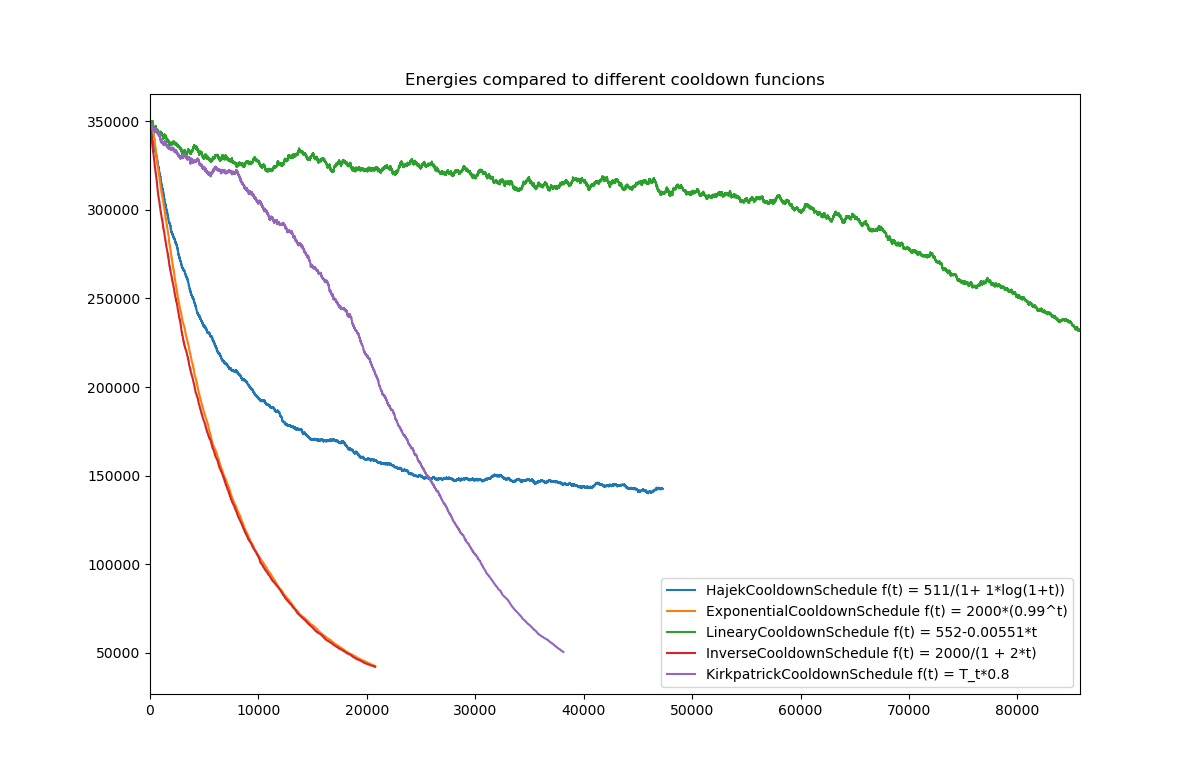
\includegraphics[width=\linewidth]{content/simulatedAnnealing/Bilder/Energy_Cooldown_compared_steps_85771.png}
    \caption{Vergleich von Abkühlfunktionen mit gesetzten Parametern
            alle mit 100000 Schritten; auf x-Achse sind erfolgreiche Schritte nach Wahrscheinlichkeitsakzeptanzfunktion
            aufgetragen}
    \label{pic:Cool Down Comparisson}
\end{figure}

%%%%%%%%%%%%%%%%%%%%%%%%%%%%%%%%%%%%%%%%%%%%%%%%%%%%%%%%%%%%%%%%%%%%%%%%%%%%%%%%%%%%%%%%%%%%%%%%%%%%%
%%%%%%%%%%%%%%%%%%%%%%% this is our cooling schedule we are going for %%%%%%%%%%%%%%%%%%%%%%%%%%%%%%%
%%%%%%%%%%%%%%%%%%%%%%%%%%%%%%%%%%%%%%%%%%%%%%%%%%%%%%%%%%%%%%%%%%%%%%%%%%%%%%%%%%%%%%%%%%%%%%%%%%%%%

\subsubsection{Kirkpatrick}
Wir haben uns bei unserem Optimierungsproblem für einen Abkühlvorgang, der in \cite{Kirkpatrick671} beschrieben wird, 
entschieden und in danach benannt. Die Abkühlfunktion hat hierbei exponentiellen Charakter. 

\begin{tcolorbox}[rightrule=3mm, rounded corners=east]
    \begin{equation}\label{eq:ExponentialKirkpatrick}
        f(t) = T_0 * pow(\alpha,t)
      \end{equation}
\end{tcolorbox}

Wobei wieder $\alpha \in [0.8; 0.99]$ und nach Auflösung der Textur zu wählen ist. Ein anderer Parameter, der nach 
Auflösung der Textur zu wählen ist, ist das Quasi-Gleichgewicht. Mit dem Quasi-Gleichgewicht lässt sich erreichen, 
dass jeder Bildabschnitt vor dem jeweiligen Abkühlen jede Temperatur durchläuft und dabei jeden Bildabschnitt davor 
bewahrt in einen lokalen Minima zu verharren.
So lässt sich in einem direkten Vergleich mit dem bloßen exponentiellen Abkühlen in Abbildung 
\ref{pic:Cool Down Comparisson} erkennen, das wir anfangs langsamer abkühlen und immer wieder auch 
höhere Energiezustände bewusst zu lassen.

\begin{figure}[H]
    \centering
    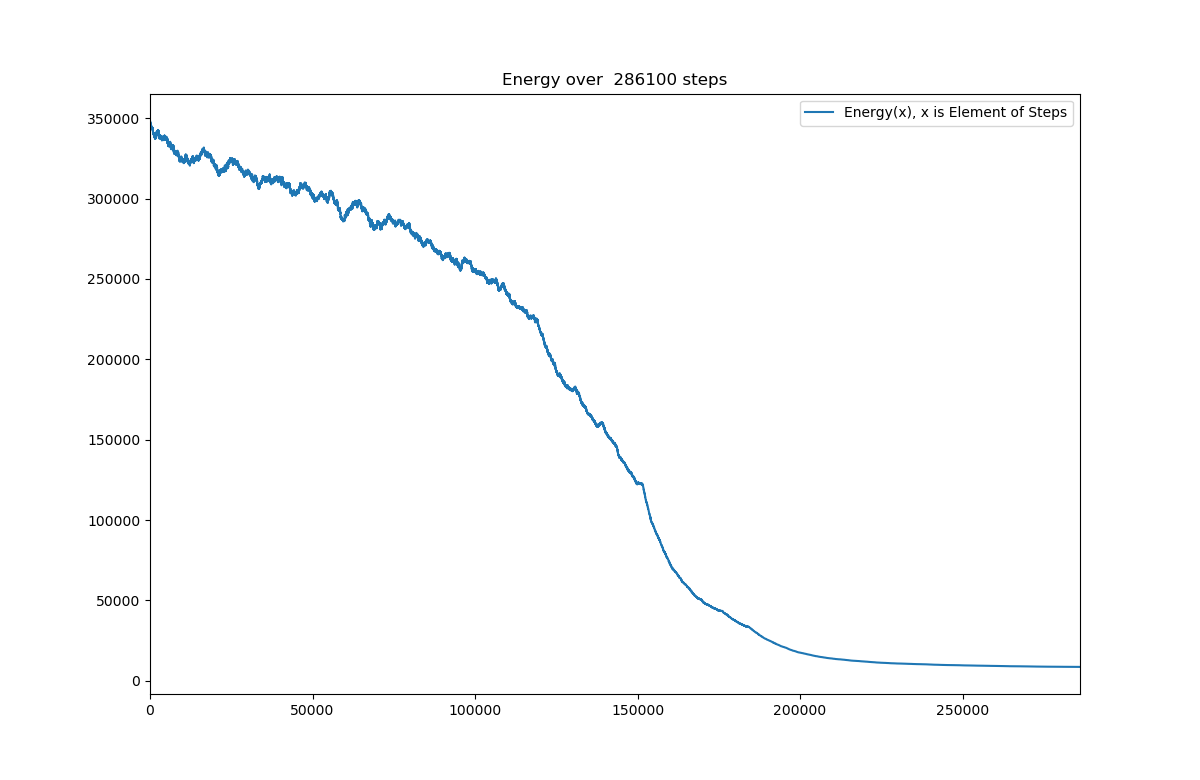
\includegraphics[width=\linewidth]{content/simulatedAnnealing/Bilder/Energy_286100_steps_KirkpatrickCooldownSchedule.png}
    \caption{Energieverlauf beim Simulated Annealing}
    \label{pic:kirkpatrick energie verlauf}
\end{figure}

Die Abbildung \ref{pic:kirkpatrick energie verlauf} verdeutlicht, dass wir durch unser Abkühlen insgesamt die 
Energiefunktion \ref{eq:pixel energy function} minimieren. Dabei akzeptieren wir in Abhängigkeit unserer Schritte,
anfangs sehr häufig und am Ende immer seltener, neben günstigeren Zuständen, auch energetische Höherwertigere.

\begin{figure}[H]
    \centering
    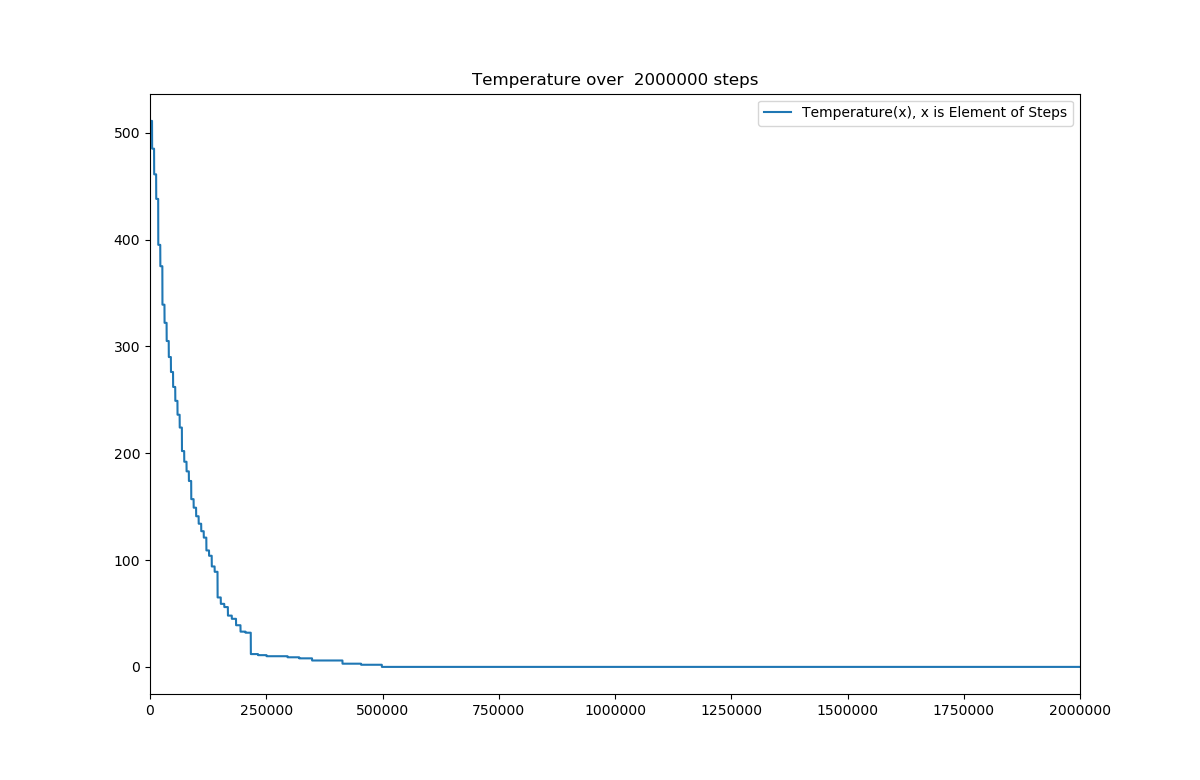
\includegraphics[width=\linewidth]{content/simulatedAnnealing/Bilder/Temperature.png}
    \caption{Temperaturverlauf}
    \label{pic:Temperaturverlauf kirkpatrick}
\end{figure}

Wir wählen die Starttemperatur (siehe Abbildung \ref{pic:Temperaturverlauf kirkpatrick}) folgendermaßen, dass 
anfangs alle Permutationen akzeptiert werden. Dazu muss die 
Akzeptanzwahrscheinlichkeitsfunktion \ref{eq:Akzeptanzwahrscheinlichkeitsfunktion} auch die energetisch
ungünstigste Permutation akzeptieren. Minimiere Argument der Exponentialfunktion \ref{fig:Exponentialfunktion}.
In unseren konkreten Fall: Maximales $\Delta_{Energy}$ bei einem 8-Bit Graustufenbild 2*255 = 510. Jeweilige 
Anpassungen müssen bei anderer Auflösung vorgenommen werden.

\begin{figure}[H]
    \centering
    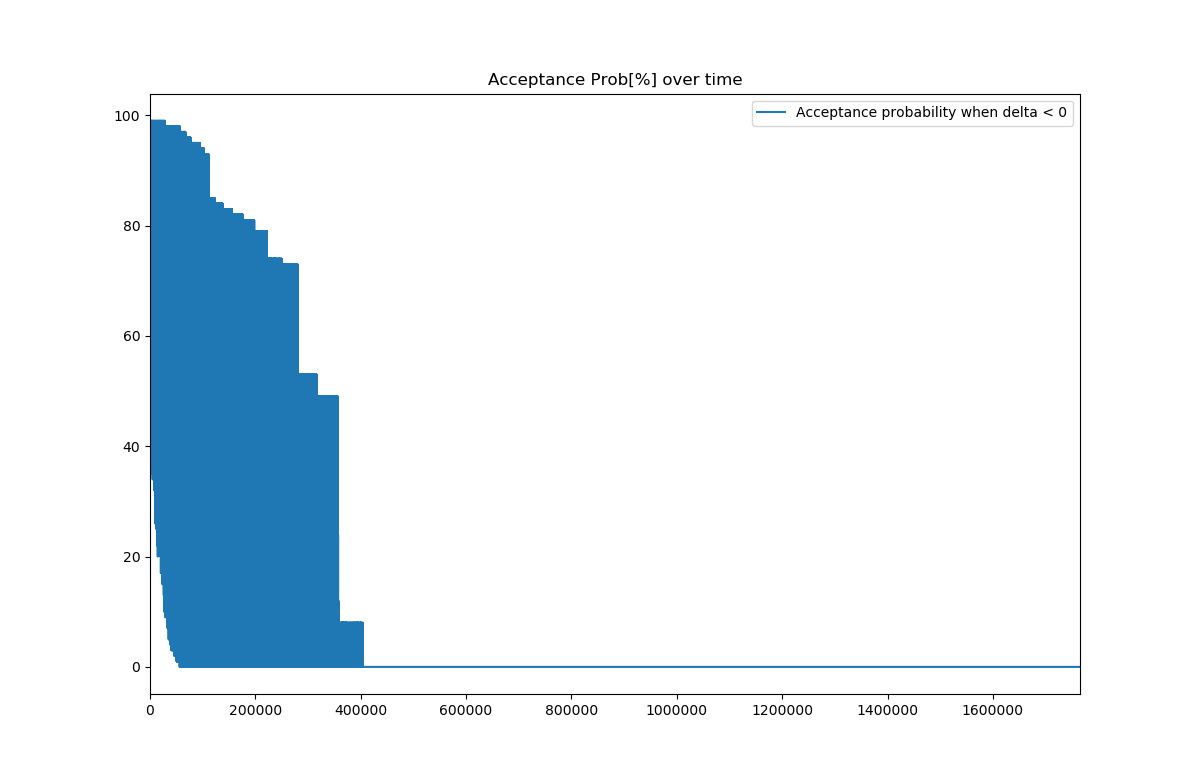
\includegraphics[width=\linewidth]{content/simulatedAnnealing/Bilder/Acceptance_Probabilities_over_time_1765297_steps_KirkpatrickCooldownSchedule.png}
    \caption{Akzeptanzfunktionsverlauf bei negativen Energiedeltas}
    \label{pic:Akzeptanzfunktionsverlauf kirkpatrick}
\end{figure}

Abbildung \ref{pic:Akzeptanzfunktionsverlauf kirkpatrick} zeigt das Aufkommen der Werte der Gleichung
\ref{eq:Akzeptanzwahrscheinlichkeitsfunktion} an. Zu Anfang gibt es keine niederen und ausschließlich 
hohe Wahrscheinlichkeiten der Akzeptanz wohingegen am Schluss keine energetisch schlechteren Permutationen 
akzeptiert werden.

\begin{figure}[H]
    \centering
    \begin{minipage}[t]{0.45\linewidth}
        \centering
        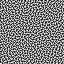
\includegraphics[interpolate=false,width=\linewidth]{content/simulatedAnnealing/Bilder/LDR_RGBA_0_64-RGBA_r_channel.png}
        \caption{Blue noise Textur 64x64}
    \end{minipage}
    \hfill
    \begin{minipage}[t]{0.45\linewidth}
        \centering
        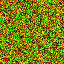
\includegraphics[interpolate=false,width=\linewidth]{content/simulatedAnnealing/Bilder/permutation_texture_295744_swapsKirkpatrickCooldownSchedule.png}
        \caption{Permutation; gespeichert in R,G-Channel einer PNG}
        \label{pic:Retargeting textur}
    \end{minipage}
\end{figure}

%%%%%%%%%%%%%%%%%%%%%%%%%%%%%%%%%%%%%%%%%%%%%%%%%%%%%%%%%%%%%%%%%%%%%%%%%%%%%%%%%%%%%%%%%%%%%%%%%%%%%%%%%%%%%%%%%%%%%%%%%%%%%%%%%%
%%%% Animate the annealing!!!!!! %%%%%%%%%%%%%%%%%%%%%%%%%%%%%%%%%%%%%%%%%%%%%%%%%%%%%%%%%%%%%%%%%%%%%%%%%%%%%%%%%%%%%%%%%%%%%%%%%
%%%%%%%%%%%%%%%%%%%%%%%%%%%%%%%%%%%%%%%%%%%%%%%%%%%%%%%%%%%%%%%%%%%%%%%%%%%%%%%%%%%%%%%%%%%%%%%%%%%%%%%%%%%%%%%%%%%%%%%%%%%%%%%%%%

\begin{figure}[H]
    \begin{tcolorbox}[boxrule=4pt,sharp corners=downhill,title=Abkühlen]
    \centering
    \begin{subfigure}[b]{0.2\linewidth}
      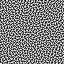
\includegraphics[width=\linewidth]{content/simulatedAnnealing/Bilder/Annealing/intermediate_applied_permutation_0_quasieqstepKirkpatrickCooldownSchedule_energy_348180-RGBA_r_channel.png}
       \caption{\nameref{ch:Content1:sec:blue noise} t}
       \label{pic:dither0}
    \end{subfigure}
    \begin{subfigure}[b]{0.2\linewidth}
      
\includegraphics[width=\linewidth]{content/simulatedAnnealing/Bilder/Annealing/intermediate_applied_permutation_1_quasieqstepKirkpatrickCooldownSchedule_energy_313012-RGBA_r_channel.png}
      \caption{313012}
      \label{pic:abkühl_schritt_1}
    \end{subfigure}
    \begin{subfigure}[b]{0.2\linewidth}
      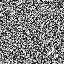
\includegraphics[width=\linewidth]{content/simulatedAnnealing/Bilder/Annealing/intermediate_applied_permutation_2_quasieqstepKirkpatrickCooldownSchedule_energy_281170-RGBA_r_channel.png}
      \caption{281170}
      \label{pic:abkühl_schritt_2}
    \end{subfigure}
    \begin{subfigure}[b]{0.2\linewidth}
        
\includegraphics[width=\linewidth]{content/simulatedAnnealing/Bilder/Annealing/intermediate_applied_permutation_3_quasieqstepKirkpatrickCooldownSchedule_energy_253330-RGBA_r_channel.png}
         \caption{253330}
         \label{pic:abkühl_schritt_3}
      \end{subfigure}

    %%%%%%%%%%%%%%%%%%%%%%%%%%%%%%%%%%%%%%%%%%%%%%%%%%%%%%%%%%%%%%%%%%%%%%%%%%%%%%%%%%%%%%%%%%%%%%%%%%%%%%
    %%%%%%%%%%%%%%%%%%%%%%%%%%%%%%% second row
    %%%%%%%%%%%%%%%%%%%%%%%%%%%%%%%%%%%%%%%%%%%%%%%%%%%%%%%%%%%%%%%%%%%%%%%%%%%%%%%%%%%%%%%%%%%%%%%%%%%%%%

    \begin{subfigure}[b]{0.2\linewidth}
        
\includegraphics[width=\linewidth]{content/simulatedAnnealing/Bilder/Annealing/intermediate_applied_permutation_4_quasieqstepKirkpatrickCooldownSchedule_energy_185486-RGBA_r_channel.png}
        \caption{185486}
        \label{pic:abkühl_schritt_4}
    \end{subfigure}
    \begin{subfigure}[b]{0.2\linewidth}
        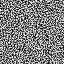
\includegraphics[width=\linewidth]{content/simulatedAnnealing/Bilder/Annealing/intermediate_applied_permutation_5_quasieqstepKirkpatrickCooldownSchedule_energy_136464-RGBA_r_channel.png}
        \caption{136464}
        \label{pic:abkühl_schritt_5}
    \end{subfigure}
    \begin{subfigure}[b]{0.2\linewidth}
        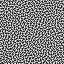
\includegraphics[width=\linewidth]{content/simulatedAnnealing/Bilder/Annealing/intermediate_applied_permutation_11_quasieqstepKirkpatrickCooldownSchedule_energy_29068-RGBA_r_channel.png}
         \caption{29068}
         \label{pic:abkühl_schritt_6}
    \end{subfigure}
    \begin{subfigure}[b]{0.2\linewidth}
        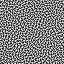
\includegraphics[width=\linewidth]{content/simulatedAnnealing/Bilder/Annealing/intermediate_applied_permutation_20_quasieqstepKirkpatrickCooldownSchedule_energy_13070-RGBA_r_channel.png}
        \caption{13070}
        \label{pic:abkühl_schritt_7}
    \end{subfigure}

    %%%%%%%%%%%%%%%%%%%%%%%%%%%%%%%%%%%%%%%%%%%%%%%%%%%%%%%%%%%%%%%%%%%%%%%%%%%%%%%%%%%%%%%%%%%%%%%%%%%%%%
    %%%%%%%%%%%%%%%%%%%%%%%%%%%%%%% third row
    %%%%%%%%%%%%%%%%%%%%%%%%%%%%%%%%%%%%%%%%%%%%%%%%%%%%%%%%%%%%%%%%%%%%%%%%%%%%%%%%%%%%%%%%%%%%%%%%%%%%%%

    \begin{subfigure}[b]{0.2\linewidth}
        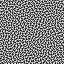
\includegraphics[width=\linewidth]{content/simulatedAnnealing/Bilder/Annealing/intermediate_applied_permutation_49_quasieqstepKirkpatrickCooldownSchedule_energy_8688-RGBA_r_channel.png}
        \caption{8688}
        \label{pic:abkühl_schritt_8}
    \end{subfigure}
    \begin{subfigure}[b]{0.2\linewidth}
        \begin{picture}(120,120)
            \put(35,50){\Huge $\approx$}
        \end{picture}
    \end{subfigure}
    \begin{subfigure}[b]{0.2\linewidth}
        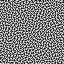
\includegraphics[width=\linewidth]{content/simulatedAnnealing/Bilder/next_dither_LDR_RGBA_0_64_r_channel.png}
        \caption{\nameref{ch:Content1:sec:blue noise} t+1}
        \label{pic:dither1}
    \end{subfigure}
    \end{tcolorbox}
    \caption{Der Prozess des Abkühlens mit jeweiliger Auswertung der Energiefunktion \ref{eq:pixel energy function}}
    \label{fig:annelaing animated}
\end{figure}

  Nachdem wir in Bild 
  \begin{itemize}
    \item[\ref{pic:dither0}] unsere \nameref{ch:Content1:sec:blue noise} Textur zum Zeitpunkt t=0 
                              haben können wir in dem Bild
    \item[\ref{pic:abkühl_schritt_1}] typische Clusterbildungen erkennen, die die Folge von 
                                    uniformen randomisierten Vertauschungen sind. Diese hatte wir bereits 
                                    im Abschnitt \ref{ch:Content1:sec:blue noise} und \ref{ch:Content1:sec:Quasi-Zufallsfolgen}
                                    besprochen. Diese Vertauschungen sind die Folge der hohen Temperatur, welche wiederrum zur Folge haben, 
                                    dass alle Vertauschungen von der Funktion \ref{eq:Akzeptanzwahrscheinlichkeitsfunktion} angenommen werden. 
                                    Die Bilder  
    \item[\ref{pic:abkühl_schritt_2}-\ref{pic:abkühl_schritt_4}] sind die Folge der abnehmenden Temperatur und der daraus folgenden geringeren 
                                    Akzeptanz schlechterer, energiereicherer Zustände. Bessere Zustände werden allerdings immer angenommen und 
                                    daher die immer bessere \nameref{ch:Content1:sec:blue noise} Verteilung. Die bessere Verteilung ist eben über 
                                    die gesamte Textur zu erkennen. Mit abnehmender Energie in den Bildern   
    \item[\ref{pic:abkühl_schritt_5}-\ref{pic:abkühl_schritt_8}] lassen wir sehr wenige/keine schlechteren Zustände mehr zu und gelangen durch 
                                    lokale Permutationen zu einer immer exakteren Verteilung.  
    \item[\ref{pic:dither1}] Zieltextur; so soll unsere Textur t nach angewandter 
                              Permutation aussehen. 
  \end{itemize}






%% ===========================


%% content.tex
%%

%% ==============
\newpage
\chapter{Temporaler Algorithmus}
\label{ch:Temporaler Algorithmus}
In diesem Abschnitt wird auf den in \cite{hal02158423} vorgestellten, temporalen Algorithmus eingegangen.
Dieser besteht grundsätzlich aus den beiden Schritten: \nameref{ch:Content2:sec:Sorting} und  
\nameref{ch:Content2:sec:Retargeting}. Wir werden die gewonnenen Erkenntnisse (siehe Kapitel \ref{ch:Grundlagen})
nutzen um eine zeitlich stabile \nameref{ch:Content1:sec:blue noise} Fehlerverteilung im Bildraum zu erreichen.
Der benutzte \nameref{ch:Content1:sec:Path Tracer} benutzt zufällig generierte Anfangswerte 
(siehe \cite{matsumoto1998mersenne}). Der darauffolgende Schritt sortiert diese Anfangswerte anhand 
einer \nameref{ch:Content1:sec:blue noise} Textur, auf die mit Hilfe einer quasi-zufälligen Sequenz 
\ref{ch:Content1:sec:Quasi-Zufallsfolgen} zugegriffen wird. Bevor diese sortierten Anfangswerte 
zum Rendern des nächsten Bildes benutzt werden durchlaufen Sie noch eine Permutation 
(siehe Abschnitt \ref{ch:Content2:sec:Retargeting}).
Desweiteren sollte man beachten, dass für diesen Algorithmus Annahmen getroffen wurden, auf deren Ursache im darauffolgenden 
Abschnitt \ref{ch:Content2:sec:a Posteriori} eingegangen wird:
Der Algorithmus arbeitet Blockweise auf den Pixeln und erwartet, dass benachbarte
Pixel innerhalb dieses Blockes den selben Wert haben. Da wir einen temporalen Algorithmus haben, soll diese Annahme 
auch über mehrere gerenderte Bilder hinweg gelten. Es sollte also beachtet werden, dass der Algorithmus z.B. nicht 
für Objektkanten oder ruckartige Bewegungen (der Kamera oder Objekte) ausgelegt ist.

\begin{figure}[H]
    \begin{subfigure}{\textwidth}
        \centering 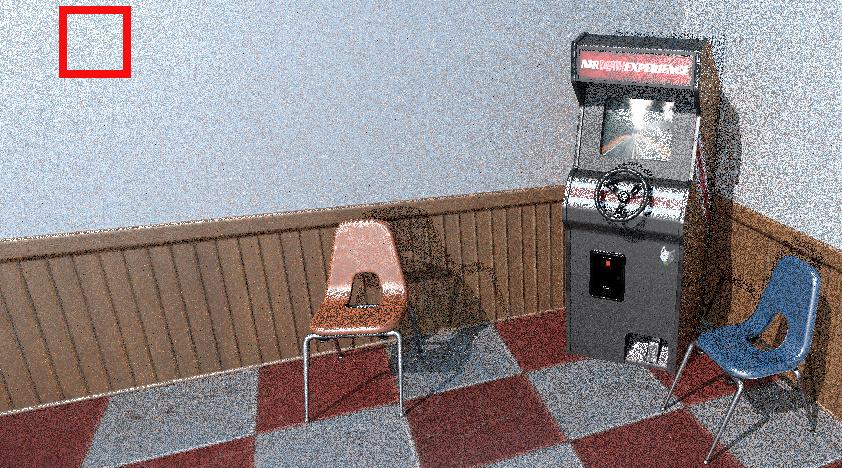
\includegraphics[width=0.7\linewidth]{content/TemporalerAlg/Bilder/WhiteNoise/white_noise_ausschnitt.png}
        \caption{Szene}
        \label{fig:Szene_Weißes Rauschen}
    \end{subfigure}
    \begin{subfigure}{0.5\textwidth}
        \centering 
\includegraphics[width=0.5\linewidth]{content/TemporalerAlg/Bilder/WhiteNoise/white_noise_64x64.jpg} 
        \caption{Szenenausschnitt}
        \label{fig:ausschnitt_Weißes_Rauschen}
    \end{subfigure}
    \begin{subfigure}{0.5\textwidth}
        \centering 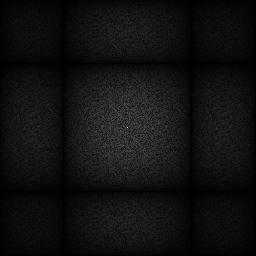
\includegraphics[width=0.5\linewidth]{content/TemporalerAlg/Bilder/WhiteNoise/white_noise_64x64_fourier.png}
        \caption{Fouriertransformierte des Ausschnitts}
        \label{fig:Fouriertransformierte_Weißes_Rauschen}
    \end{subfigure}
        \caption{Ausgangssituation; Erzeugtes Bild mit zufälligen Seeds ohne temp. Alg.}
        \label{fig:Path Tracer mit zufälligen Seeds}
\end{figure}

In Abbildung \ref{fig:Path Tracer mit zufälligen Seeds} sehen wir die Ausgabe des \nameref{ch:Content1:sec:Path Tracer}
mit zufälligen Anfangswerten(Mersenne-Twister) weder mit dem Sortier \ref{ch:Content2:sec:Sorting} noch dem 
\nameref{ch:Content2:sec:Retargeting} Schritt. Der Szenenausschnitt lässt deutliche Clusterbildungen erkennen und auch
die Betrachtung des Spektrums lässt auf eine white noise \ref{pic:white noise} Verteilung schließen.

%% ==============

%% ===========================
\newpage
\newpage
\section{A Posteriori}
\label{ch:Content2:sec:a Posteriori}
Der nun behandelte temporale Algorithmus von \cite{hal02158423} beruht 
im Gegensatz zu \cite{georgiev2016blue} auf \textit{nachträglichen} 
Annahmen. Welches zur Folge hat, dass die Dimension unseres Path Tracers
\nameref{ch:Content1:sec:PathTracer}, sowie die Stichprobenanzahl einhergehen 
mit der Verteilung der Integrationsfehler als blue noise im Bildraum.
Die zu Grunde liegenden Annahmen sollen nun im Folgenden untersucht werden.

\subsection{Theoretische Grundlage}

Im Kapitel \nameref{ch:Content1:sec:PathTracer} haben wir gesehen, dass 
wir den Wert eines Pixels (i,j) klassischerweise mit einem zufälligen
Startwert durch eine Monte-Carlo Integration erhalten. Wir betrachten im
Folgenden eine (theoretische) Menge von allen möglichen Werten eines 
Pixels, welche durch alle möglichen Startwerte generiert wurde.
In \nameref{eq:Pixel Schätzung Wahrscheinlichkeitsdichtefunktion} ist die Wahrscheinlichkeitsdichtefunktion
$h_{ij}$ aufgetragen, als eine Funktion über alle möglichen Werte 
$I_{ij}$ eines Pixels (i,j).

\begin{equation}\label{eq:Pixel Schätzung Wahrscheinlichkeitsdichtefunktion}
    H_{ij}([I_{Anfang},I_{Ende}]) = \int_{I_{Anfang}}^{I_{Ende}} h_{ij} dI
\end{equation}

Verfolgt man beispielhaft die Werte eines Pixels über 9 frames bei unseren Path Tracer 
basierend auf \cite{Benty18}, so ergibt es sich zur Anschauung wie folgt:

\begin{figure}[H]

    \begin{subfigure}{\textwidth}
        \centering 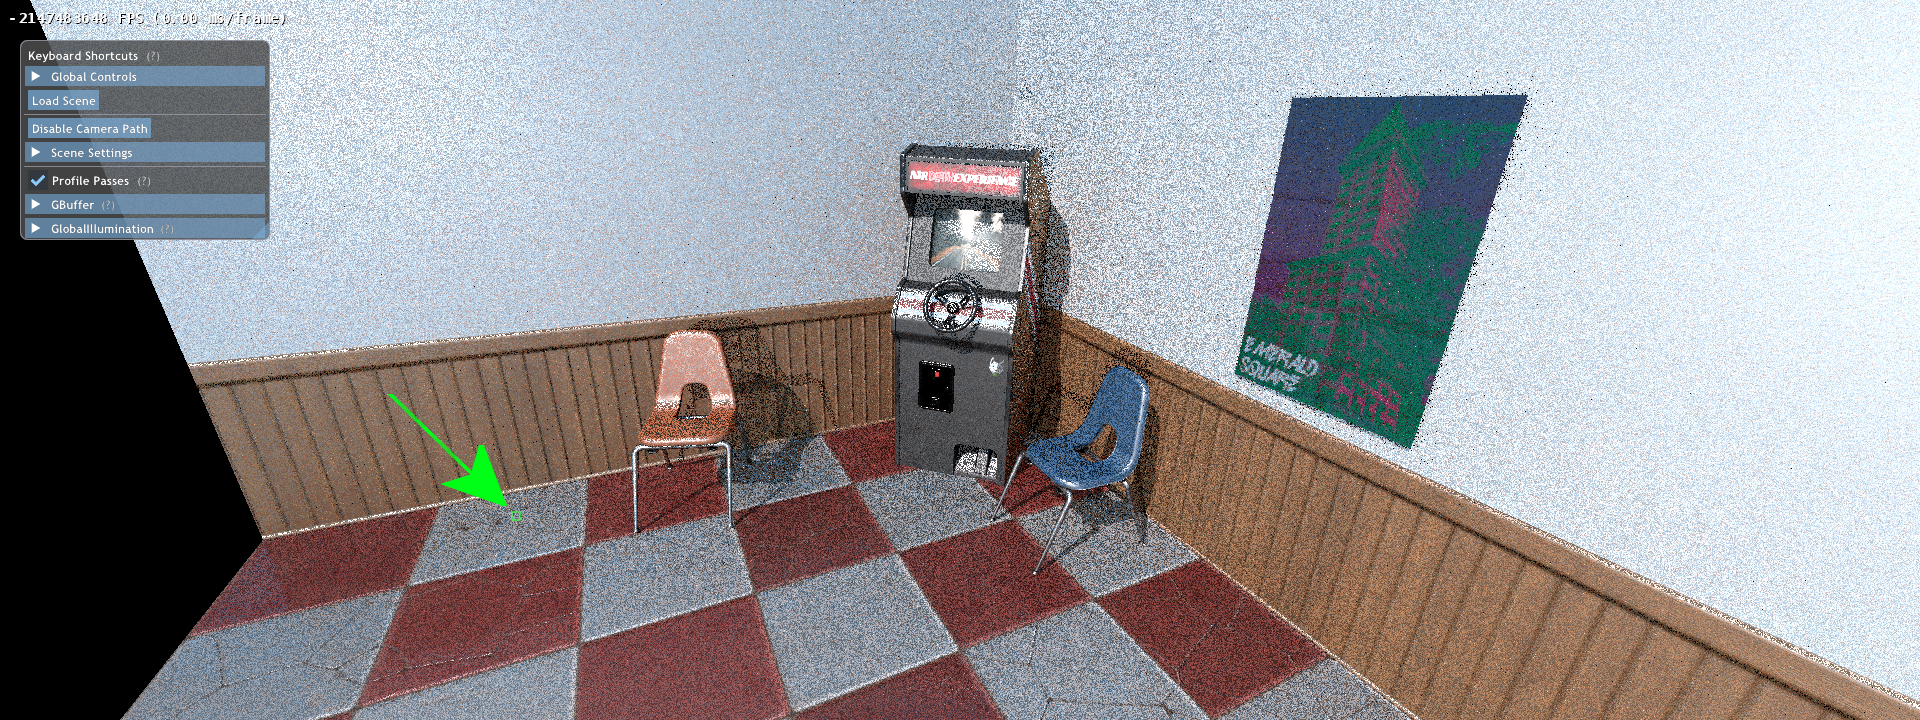
\includegraphics[width=0.6\linewidth]{content/TemporalerAlg/Bilder/APosteriori/frame_t_whitenosie2.0.png} 
        \caption{Szenenausschnitt}
        \label{fig:szene_pixel_position_512x512}
    \end{subfigure}

    \begin{subfigure}{0.5\textwidth}
        \centering 
\includegraphics[width=0.6\linewidth]{content/TemporalerAlg/Bilder/APosteriori/pixel_512x512_strip.png} 
        \caption{Werte des Pixels an Position 512x512 im zeitlichen Verlauf (Rote Markierung)}
        \label{fig:ausschnitt_pixelstrip}
    \end{subfigure}
    \begin{subfigure}{0.5\textwidth}
            \centering
            \def\svgwidth{\columnwidth}
            \import{content/TemporalerAlg/Bilder/APosteriori/}{histogram_of_estimates.pdf_tex}
            \label{histogramOfEstimates}
            \caption{Histogram der Pixelschätzungen}
    \end{subfigure}
        \caption{Pixelwerte an Position 512x512(grüne Markierung) in aufeinanderfolgenden Zeitschritten}
        \label{fig:Pixelwerte}

\end{figure}

Allerding betrachten wir die theoretische Menge aller Werte. Demnach können wir das Rendern 
eines jeden konkreten Pixels als die Wahl eines Wertes anhand der Wahrscheinlichkeitsdichtefunktion
sehen.

Daraus lässt sich die Gleichbedeutung zweier Aussagen begründen:
Das Rendern des Pixels (i,j) und das Wählen eines Pixelswertes $I_{ij}$
von unser zuvor formulierten Wahrscheinlichkeitsdichtefunktion $h_{ij}$.

\begin{equation}\label{eq:inverse Funktion}
    I_{ij} = H_{ij}^{-1}(x), x \in [0,1]
\end{equation}

Nun betrachte man die Werte für x in \nameref{eq:inverse Funktion} als im Bildraum
blue noise verteilte Zahlen. Daraus folgt, dass die resultierenden
Integrationsfehler auch als blue noise im Bildraum verteilt sind.


\subsection{Praktische Durchführung}
Die Berechnung des vollständigen Histogramms ist für eine Echtzeitanwendung
zu kostenintensiv. Stattdessen könnte man auch die dadurch beanspruchte 
Rechenleistung auf z.B mehrere Samples pro Pixel verteilen.
Stattdessen werden wir in dem temporalen Algorithmus von \cite{hal02158423}
das Histogramm mit dem vorherigen Frame approximieren. 
Bereits vorherige Arbeiten \cite{Schied:2018:GER:3273023.3233301} haben die 
Wirksamkeit eines solchen temporalen Ansatzes(Zugriff auf das vorherige Frame)
gezeigt. Die Approximation des Histogramms erfolgt dadurch mit dem $Frame_{t}$ 
für $Frame_{t+1}$,indem umliegende Pixel in das Histogramm aufgenommen werden.
Offensichtliche Konsequenzen dieser blockweisen Verarbeitung sind schlechte blue noise 
Fehlerverteilungen im Bildraum bei sich stark ändernden Bildausschnitten
(so z.B. bei Objektkanten), da dort die Annahme, dass eine ähnliche Oberfläche
zur Farbgebung beiträgt verletzt wird.


\begin{algorithm}[H]
    \caption{Benutzung unser zwei vorberechneten Texturen: Blue Noise und Retarget}
    \begin{algorithmic}[1]
        \State $bluenoise_{t}$(i,j) = $bluenoise_{0}$(i + $\alpha$t, j + $\beta$t); 
        \State $retarget_{t}$(i,j) = $retarget_{0}$(i + $\alpha$t, j + $\beta$t) + ($\alpha$t, $\beta$t)
    \end{algorithmic}
    \label{alg:Benutzung vorberechneter Texturen}
\end{algorithm}

\begin{figure}[H]
    \centering
    \begin{subfigure}[b]{0.4\textwidth}
        \centering 
\includegraphics[interpolate=false, width=\linewidth]{content/TemporalerAlg/Bilder/APosteriori/homogener_ausschnitt_blocksize.png}
        \label{fig:homogener Pixelblock}
        \caption{homogener Pixelblock}
    \end{subfigure}
    ~ %add desired spacing between images, e. g. ~, \quad, \qquad, \hfill etc. 
      %(or a blank line to force the subfigure onto a new line)
    \begin{subfigure}[b]{0.4\textwidth}
        \centering 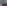
\includegraphics[interpolate=false,width=\linewidth]{content/TemporalerAlg/Bilder/APosteriori/inhomogener_ausschnitt_blocksize.png}
        \label{fig:Inhomogener Pixelblock}
        \caption{inhomogener Pixelblock}
    \end{subfigure}

    \caption{Pixelblöcke bei (in-)homogenen Flächen}\label{fig:Pixelblöcke}
\end{figure}
%% ===========================



%% ===========================
\newpage
\newpage
\section{Sorting}
\label{ch:Content2:sec:Sorting}
\todo{replace dummy code with correct code}
\cite{hal-02158423}
\begin{algorithm}
    \caption{\textbf{Sortier Schritt t} nach dem Rendern von Frame t
    und vor dem Rendern von Frame t+1}
    \begin{algorithmic}[1]
        \STATE pixel \textbf{consists of} value,index;
        \STATE List framePixelsIntensities, noiseIntensities;
        \STATE List L $\leftarrow$ pixels in block
        \STATE //init lists
        \FORALL{(i,j) $\leftarrow$ L} 
        \STATE framePixelsIntensities(i,j) = pixelIntensity(frame(i,j));
        \STATE noiseIntensities(i,j) = pixelIntensity(blueNoise(i,j));
        \ENDFOR \newline
        
        \STATE //sort the two lists by means of intensities
        \STATE sort(framePixelsIntensities);
        \STATE Sort(noiseIntensities); \newline

        \STATE //now we reorder our seeds hence the sorted lists
        \FORALL{$i = 1 .. numberOfPixelsPerBlock$}
        \STATE $sortedSeeds(noiseIntensities.getIndex(i)) = incomingSeeds(framePixelIntensities.getIndex(i))$;
        \ENDFOR
    \end{algorithmic}
    \label{alg:Sortier}
\end{algorithm}
%% ===========================



%% ===========================
\newpage
\newpage
\section{Retargeting}
\label{ch:Content2:sec:Retargeting}
Zu Grunde liegender Sinn dieses Schrittes: Vertauschen der Seeds, die 
verteilt sind wie $BlueNoise_{t}$ , aufgrund des zuvor ausgeführten Sortierschrittes \ref{ch:Content2:sec:Sorting}
, sodass Sie verteilt sind wie die Textur
$BlueNoise_{t+1}$. Aufgrund dessen haben wir eine Aufsummierung der
blue noise Fehlerverteilungen über die ersten paar Frames(siehe \nameref{fig:Retargeting_And_Sorting_Szene_t1}).

\begin{algorithm}[H]
    \caption{\textbf{Retargeting Schritt}}
    \begin{algorithmic}[1]
        \State //permutation indices from precomputed texture
        \State $retaget_{t}$ = retarget\_texure[calc\_correct\_offset()];
        
        \State $retargetedSeeds(old\_id + retaget_{t}) = incomingSeeds(old\_id);$
        
    \end{algorithmic}
    \label{alg:retargetingAlg}
\end{algorithm}

\begin{figure}[H]\label{pic:Permutation}
    \centering
    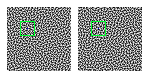
\includegraphics[width=0.5\linewidth]{content/simulatedAnnealing/Bilder/Permutation.png}
    \caption{Permutation}
\end{figure}

\newpage
%%%%%%%%%%%%%%%%%%%%%%%%%%%%%%%%%%%%%%%%%%%%%%%%%%%%%%%%%%%%
%%%%%%%%%% Beginning the Sequence of getting to blue noise from white noise
%%%%%%%%%%%%%%%%%%%%%%%%%%%%%%%%%%%%%%%%%%%%%%%%%%%%%%%%%%%%
\label{fig:Retargetbilderstrecke}
\begin{figure}[H]

    \begin{subfigure}{\textwidth}
        \centering 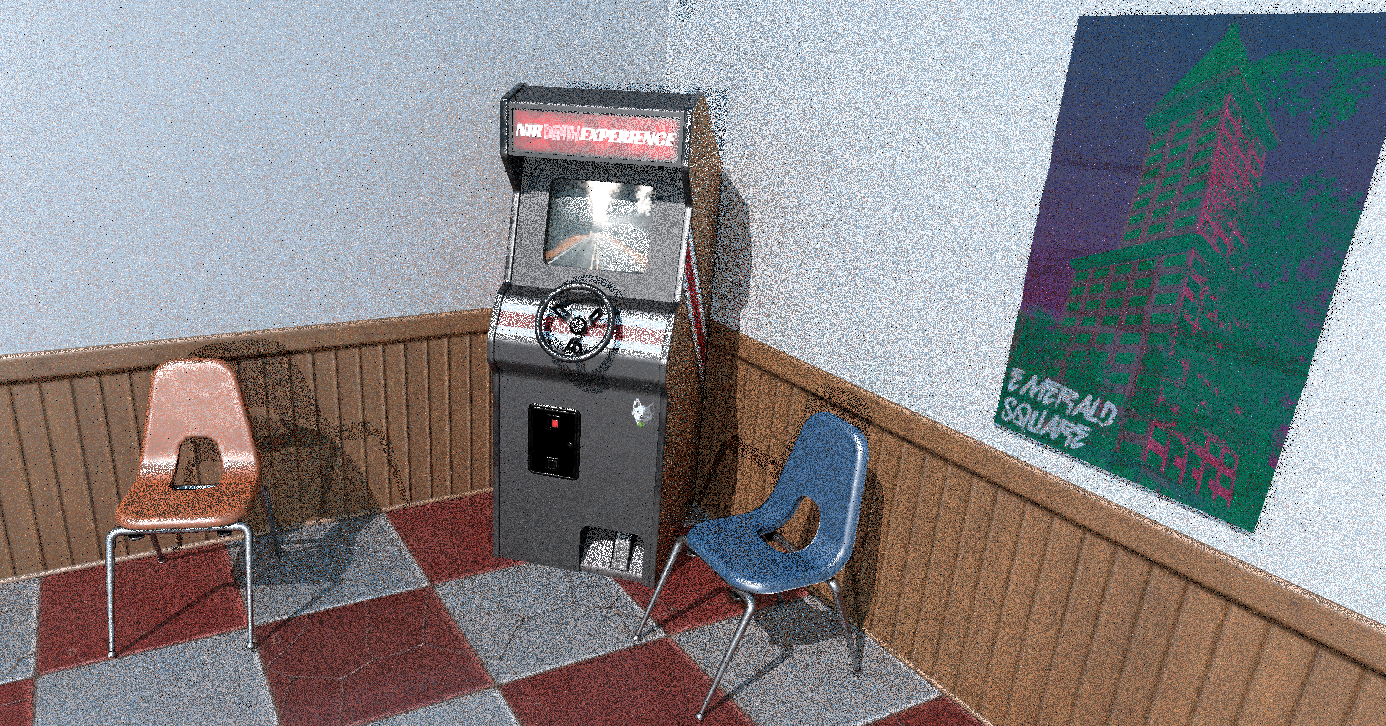
\includegraphics[scale=.25]{content/TemporalerAlg/Bilder/Retargeting/Screenshots/seed_debug_3.0_selection.png}
        \caption{Szene}
        \label{fig:Retargeting_And_Sorting_Szene_t1}
    \end{subfigure}
    \begin{subfigure}{0.5\textwidth}
        \centering 
\includegraphics[width=0.4\linewidth]{content/TemporalerAlg/Bilder/Retargeting/Screenshots/seed_debug_3.0_ausschnitt.png} 
        \caption{Szenenausschnitt}
        \label{fig:Retargeting_And_Sorting_ausschnitt_t1}
    \end{subfigure}
    \begin{subfigure}{0.5\textwidth}
        \centering 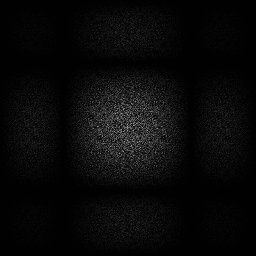
\includegraphics[width=0.4\linewidth]{content/TemporalerAlg/Bilder/Retargeting/Screenshots/Spektren/seed_debug_3.0_ausschnitt.png}
        \caption{Fouriertransformierte des Ausschnitts}
        \label{fig:Retargeting_And_Sorting_Fouriertransformierte_t1}
    \end{subfigure}
        \caption{Zeitpunkt t=1}
        \label{fig:Retargeting_And_Sorting_Verlauf_t1}
\end{figure}

\begin{figure}[H]
    \begin{subfigure}{\textwidth}
        \centering 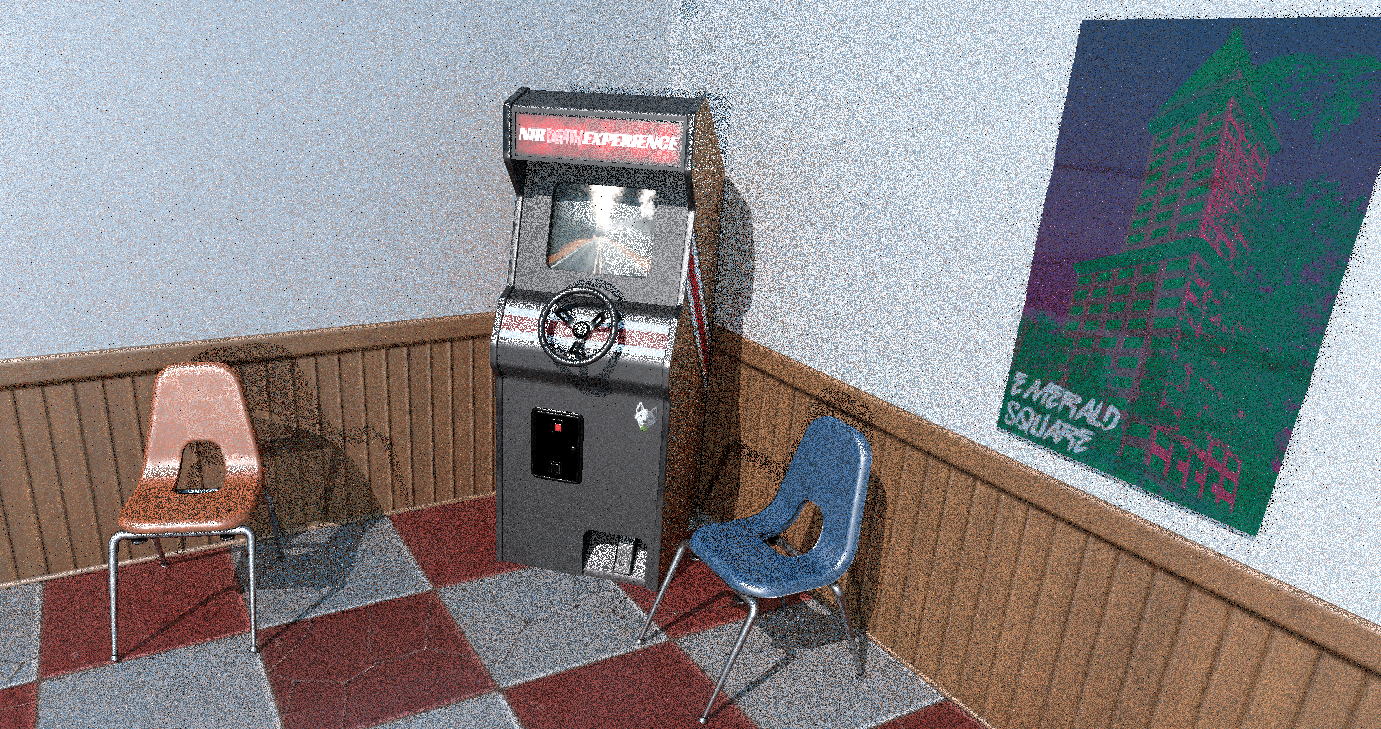
\includegraphics[scale=.25]{content/TemporalerAlg/Bilder/Retargeting/Screenshots/seed_debug_4.0_selection.png}
        \caption{Szene}
        \label{fig:Retargeting_And_Sorting_Szene_t2}
    \end{subfigure}
    \begin{subfigure}{0.5\textwidth}
        \centering
\includegraphics[width=0.4\linewidth]{content/TemporalerAlg/Bilder/Retargeting/Screenshots/seed_debug_4.0_ausschnitt.png} 
        \caption{Szenenausschnitt}
        \label{fig:Retargeting_And_Sorting_ausschnitt_t2}
    \end{subfigure}
    \begin{subfigure}{0.5\textwidth}
        \centering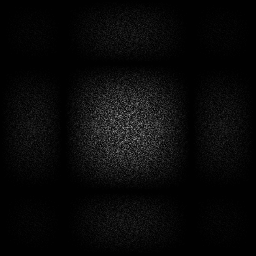
\includegraphics[width=0.4\linewidth]{content/TemporalerAlg/Bilder/Retargeting/Screenshots/Spektren/seed_debug_4.0_ausschnitt.png}
        \caption{Fouriertransformierte des Ausschnitts}
        \label{fig:Retargeting_And_Sorting_Fouriertransformierte_t2}
    \end{subfigure}
        \caption{Zeitpunkt t=2}
        \label{fig:Retargeting_And_Sorting_Verlauf_t2}
\end{figure}

\begin{figure}[H]
    \begin{subfigure}{\textwidth}
        \centering 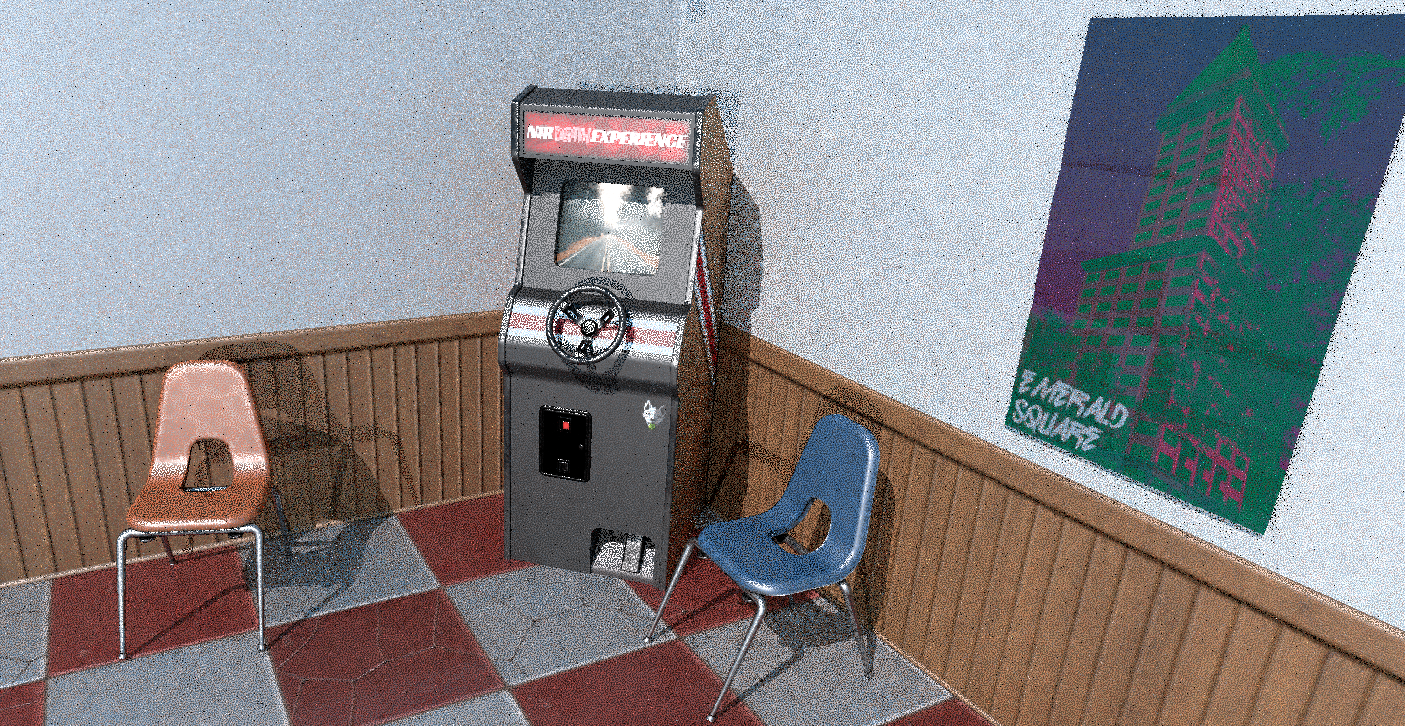
\includegraphics[scale=.25]{content/TemporalerAlg/Bilder/Retargeting/Screenshots/seed_debug_5.0_selection.png}
        \caption{Szene}
        \label{fig:Retargeting_And_Sorting_Szene_t3}
    \end{subfigure}
    \begin{subfigure}{0.5\textwidth}
        \centering
\includegraphics[width=0.4\linewidth]{content/TemporalerAlg/Bilder/Retargeting/Screenshots/seed_debug_5.0_ausschnitt.png} 
        \caption{Szenenausschnitt}
        \label{fig:Retargeting_And_Sorting_ausschnitt_t3}
    \end{subfigure}
    \begin{subfigure}{0.5\textwidth}
        \centering
\includegraphics[width=0.4\linewidth]{content/TemporalerAlg/Bilder/Retargeting/Screenshots/Spektren/seed_debug_5.0_ausschnitt.png}
        \caption{Fouriertransformierte des Ausschnitts}
        \label{fig:Retargeting_And_Sorting_Fouriertransformierte_t3}
    \end{subfigure}
        \caption{Zeitpunkt t=3}
        \label{fig:Retargeting_And_Sorting_Verlauf_t3}
\end{figure}

\begin{figure}[H]
    \begin{subfigure}{\textwidth}  
        \centering 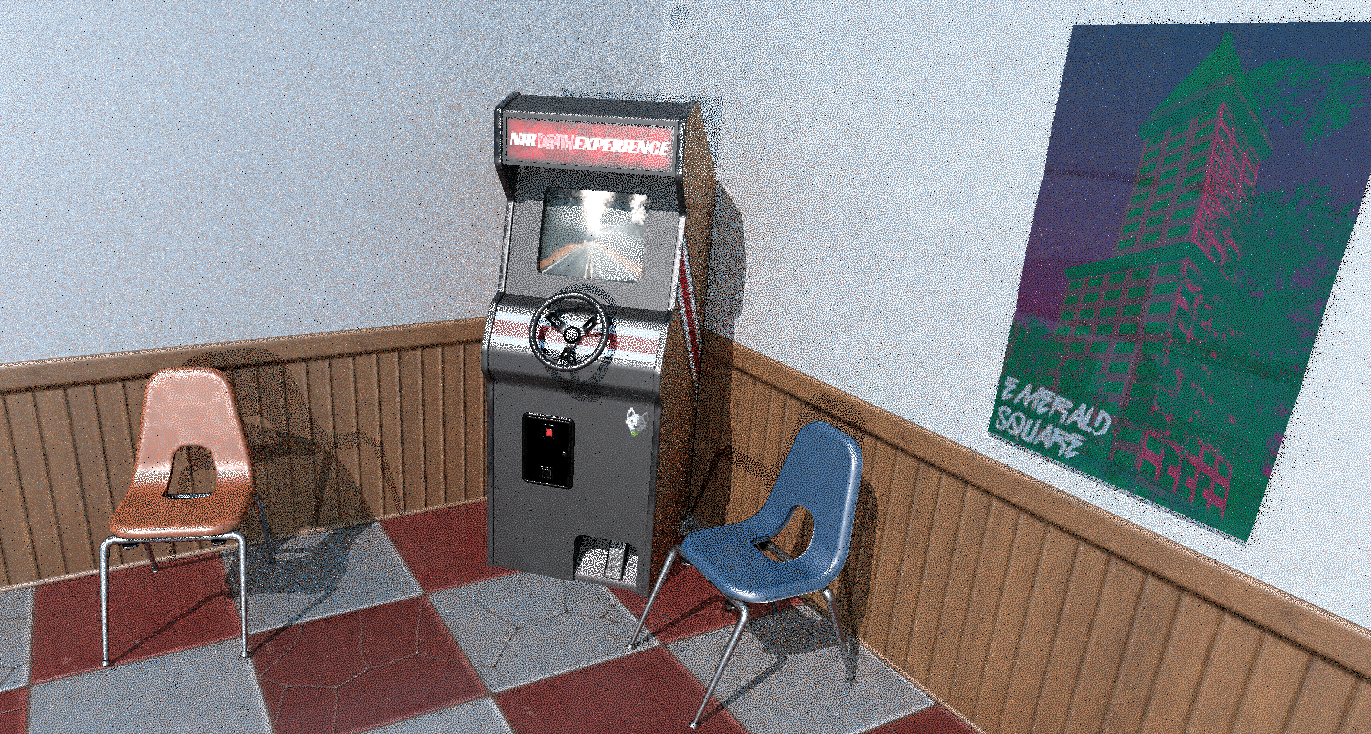
\includegraphics[scale=.25]{content/TemporalerAlg/Bilder/Retargeting/Screenshots/seed_debug_6.0_selection.png}
        \caption{Szene}
        \label{fig:Retargeting_And_Sorting_Szene_t4}
    \end{subfigure}
    \begin{subfigure}{0.5\textwidth}
        \centering
\includegraphics[width=0.4\linewidth]{content/TemporalerAlg/Bilder/Retargeting/Screenshots/seed_debug_6.0_ausschnitt.png} 
        \caption{Szenenausschnitt}
        \label{fig:Retargeting_And_Sorting_ausschnitt_t4}
    \end{subfigure}
    \begin{subfigure}{0.5\textwidth}
        \centering
\includegraphics[width=0.4\linewidth]{content/TemporalerAlg/Bilder/Retargeting/Screenshots/Spektren/seed_debug_6.0_ausschnitt.png}
        \caption{Fouriertransformierte des Ausschnitts}
        \label{fig:Retargeting_And_Sorting_Fouriertransformierte_t4}
    \end{subfigure}
        \caption{Zeitpunkt t=4}
        \label{fig:Retargeting_And_Sorting_Verlauf_t4}
\end{figure}

\begin{figure}[H]
    \begin{subfigure}{\textwidth}   
        \centering 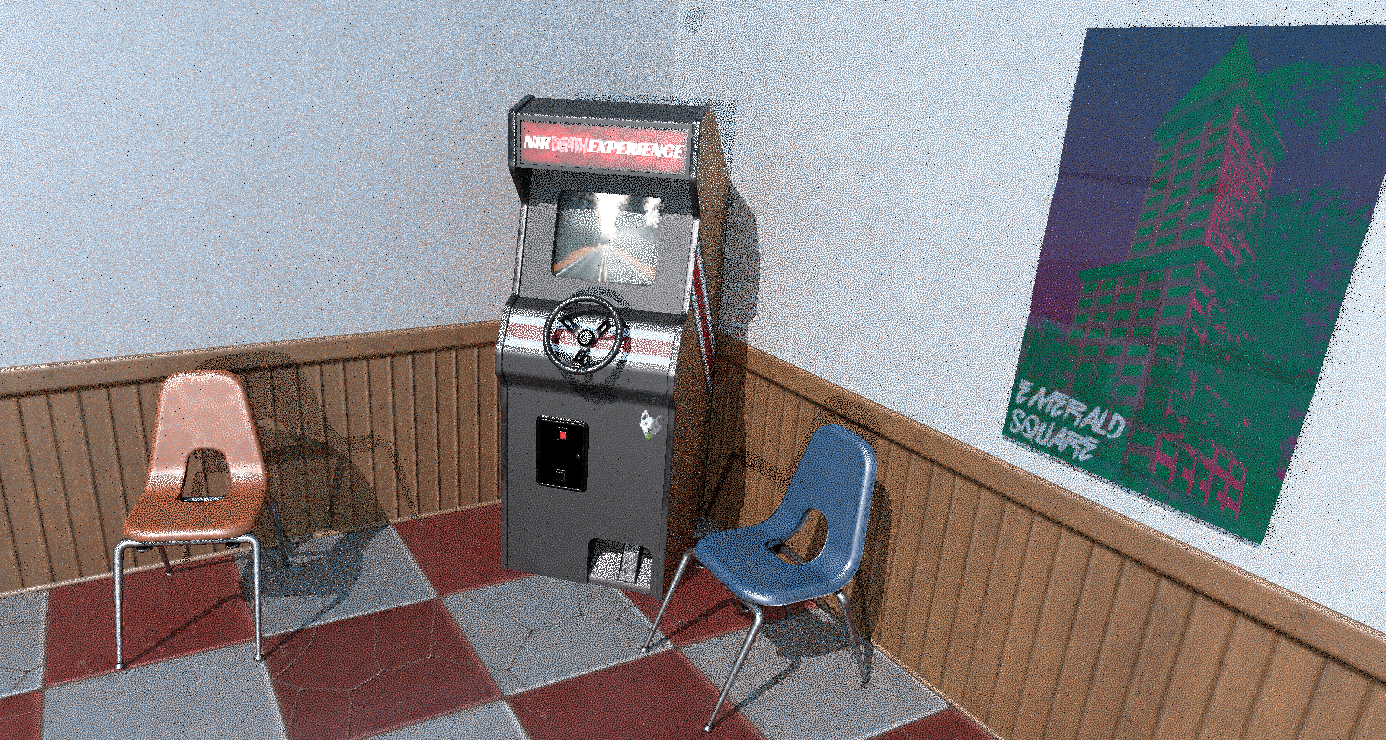
\includegraphics[scale=.25]{content/TemporalerAlg/Bilder/Retargeting/Screenshots/seed_debug_7.0_selection.png}
        \caption{Szene}
        \label{fig:Retargeting_And_Sorting_Szene_t5}
    \end{subfigure}
    \begin{subfigure}{0.5\textwidth}
        \centering
\includegraphics[width=0.4\linewidth]{content/TemporalerAlg/Bilder/Retargeting/Screenshots/seed_debug_7.0_ausschnitt.png} 
        \caption{Szenenausschnitt}
        \label{fig:Retargeting_And_Sorting_ausschnitt_t5}
    \end{subfigure}
    \begin{subfigure}{0.5\textwidth}
        \centering\includegraphics[width=0.4\linewidth]{content/TemporalerAlg/Bilder/Retargeting/Screenshots/Spektren/seed_debug_7.0_ausschnitt.png}
        \caption{Fouriertransformierte des Ausschnitts}
        \label{fig:Retargeting_And_Sorting_Fouriertransformierte_t5}
    \end{subfigure}
        \caption{Zeitpunkt t=5}
        \label{fig:Retargeting_And_Sorting_Verlauf_t5}
\end{figure}

\begin{figure}[H]
    \begin{subfigure}{\textwidth}   
        \centering \includegraphics[scale=.25]{content/TemporalerAlg/Bilder/Retargeting/Screenshots/seed_debug_8.0_selection.png}
        \caption{Szene}
        \label{fig:Retargeting_And_Sorting_Szene_t6}
    \end{subfigure}
    \begin{subfigure}{0.5\textwidth}
        \centering\includegraphics[width=0.4\linewidth]{content/TemporalerAlg/Bilder/Retargeting/Screenshots/seed_debug_8.0_ausschnitt.png} 
        \caption{Szenenausschnitt}
        \label{fig:Retargeting_And_Sorting_ausschnitt_t6}
    \end{subfigure}
    \begin{subfigure}{0.5\textwidth}
        \centering\includegraphics[width=0.4\linewidth]{content/TemporalerAlg/Bilder/Retargeting/Screenshots/Spektren/seed_debug_8.0_ausschnitt.png}
        \caption{Fouriertransformierte des Ausschnitts}
        \label{fig:Retargeting_And_Sorting_Fouriertransformierte_t6}
    \end{subfigure}
        \caption{Zeitpunkt t=6}
        \label{fig:Retargeting_And_Sorting_Verlauf_t6}
\end{figure}

\begin{figure}[H]
    \begin{subfigure}{\textwidth}   
        \centering \includegraphics[scale=.25]{content/TemporalerAlg/Bilder/Retargeting/Screenshots/seed_debug_9.0_selection.png}
        \caption{Szene}
        \label{fig:Retargeting_And_Sorting_Szene_t7}
    \end{subfigure}
    \begin{subfigure}{0.5\textwidth}
        \centering\includegraphics[width=0.4\linewidth]{content/TemporalerAlg/Bilder/Retargeting/Screenshots/seed_debug_9.0_ausschnitt.png} 
        \caption{Szenenausschnitt}
        \label{fig:Retargeting_And_Sorting_ausschnitt_t7}
    \end{subfigure}
    \begin{subfigure}{0.5\textwidth}
        \centering\includegraphics[width=0.4\linewidth]{content/TemporalerAlg/Bilder/Retargeting/Screenshots/Spektren/seed_debug_9.0_ausschnitt.png}
        \caption{Fouriertransformierte des Ausschnitts}
        \label{fig:Retargeting_And_Sorting_Fouriertransformierte_t7}
    \end{subfigure}
        \caption{Zeitpunkt t=7}
        \label{fig:Retargeting_And_Sorting_Verlauf_t7}
\end{figure}


%% ===========================


%% ===========================
\newpage
\section{Rechenaufwand}
\label{ch:Content2:sec:Rechenaufwand}
Da unsere Ressourcen beschränkt sind und trotz Hardwarebeschleunigung immer noch viel Rechenzeit eines Frames auf die globale Beleuchtung entfällt,
ist es von Bedeutung, dass unser temporaler Algorithmus keinen signifikanten zusätzlichen Aufwand schafft.
Mit einem Großteil der Rechenzeit, der auf die Berechnung des GBuffers und der globalen Beleuchtung fällt sind wir hingegen 
mit den Schritten Sorting und Retargeting (+ temporal Reprojection) sowohl auf  CPU als auf GPU Seite im niedrigen Prozentbereich.
Dabei wurde hier eine Blockgröße (siehe Abschnitt \ref{subsec:Blockgröße}) von B = 64 verwendet. Bei einer kleineren Blockgröße von B = 16, welche 
bereits gute Ergebnisse liefert, reduziert sich der Aufwand auf ein Viertel. 
\par
\newcolumntype{Y}{>{\raggedleft\arraybackslash}X}% see tabularx
%\tcbset{enhanced,fonttitle=\bfseries\large,fontupper=\normalsize\sffamily,
%colback=yellow!10!white,colframe=red!50!black,colbacktitle=red!30!white,
%coltitle=black,center title}
\begin{figure}[H]
    \begin{tcolorbox}[title=Rechenaufwand]
        \begin{tcolorbox}[tabularx={X|Y|Y},title=Pipeline, colbacktitle=yellow!50!red, coltitle=white]
            \textbf{Stufen}                                     &  \textbf{Rechenzeit(ms/\%)} CPU & \textbf{Rechenzeit(ms/\%)} GPU \\\hline\hline
            \textbf{Gesamt}                                     &  29.55/100\%                    & 19.04/100\%\\\hline
            GBuffer                                             &  06.48/21.91\%                  & 01.30/6,83\%\\\hline
            Retargeting(+ optionale temporale Reprojektion)     &  01.12/3.8\%                    & 00.11/0.57\%\\\hline
            GGXGlobalIllumination                               &  21.20/71.74\%                  & 15.51/81,46\%\\\hline\hline
            Sorting(B=64)                                       &  00.75/2,53\%                   & 02.12/11,13\%\\\hline\hline
            \textbf{Nicht in Gesamt}                            &                                 &              \\\hline\hline
            Sorting(B=16)                                       &  00.75                          & 00.55        \\\hline\hline
        \end{tcolorbox}  
        \tcblower
        \begin{tcolorbox}[tabularx={X|Y|Y},title=Vorberechnungen, colbacktitle=yellow!50!red, coltitle=white]
            \textbf{Vorberechnung}        &  \textbf{Rechenzeit(m)}    &  \textbf{Fehler(raw/\%)}\\\hline\hline
            Retargeting                   &  17,07                     &  10714 $\approx$ 3.07\%\\\hline
            Retargeting                   &  35,36                     &  9444 $\approx$ 2,71\%\\\hline
            Temporale Projizieren         &  194,7                     &  $\approx$ 10000\\\hline\hline
        \end{tcolorbox}  
    \end{tcolorbox}
    \caption{Rechenzeiten die auf die einzelnen Stages fallen}
    \medskip
    \small
    * Hardware: AMD Ryzen 5 2600X, NVIDIA GeForce RTX 2060 SUPER\newline
    * Fehler: Anteil orientiert sich am Anfangsfehler von 348180 $\rightarrow$ Summe von pixelweise Differenz Blue Noise(t=0) und Blue Noise(t=1) 
\end{figure}

Um zu einem Ergebnis wie in Figur \ref{fig:annelaing animated}(siehe Abschnitt \nameref{ch:Content2:sec:Simulated Annealing}) zu kommen, braucht man $\approx17$ Minuten. 
Diese Berechnung liefert ein gutes Ergebnis bei akzeptablen Rechenaufwand. Für einen Fehler von (minimale Verbesserung) sind bereits $\approx17$ Minuten 
nötig.

%%%%%%%%%%%%%%%%%%%
%%%%% storage usage
%%%%%%%%%%%%%%%%%%%
Wie speichern unsere Anfangswerte in einer 1920x1080 32-Bit-Textur. Die \nameref{ch:Content1:sec:blue noise} Textur innerhalb des \nameref{ch:Content2:sec:Sorting} Schrittes 
ist eine 64x64 32-Bit Textur. Die Retarget-Textur benutzt eine 64x64 16-Bit Textur. Das temporale Projizieren benutzt 11 solcher Texturen.
\begin{figure}[H]
    \begin{tcolorbox}[tabularx={X|Y},title=Speicherbedarf, colbacktitle=yellow!50!red, coltitle=white]
        \textbf{Pipelinestage}  &  \textbf{Speicherbedarf/KB} \\\hline\hline
        Sorting                 &  16,1                     \\\hline
        Retargeting             &  12,1                    \\\hline
        Temporale Reprojektion  &  133,1                    \\\hline
        Anfangswerte(Seeds)     &  7920                     \\\hline\hline
        \textbf{Gesamt}         &  \textbf{8226,5}           \\\hline\hline                
    \end{tcolorbox}
    \caption{Speicherdarf}
\end{figure}

Die Texturen für das Retargeting sowie für das temporale Projizieren wurden unkomprimiert verwendet. Dabei würde dies ein weiteres hohes
Speichereinsparpotenzial bieten. Bei den 8 Bit pro Farbkanal stehen uns 256 Werte zum Abspeichern bereit. Dabei benutzen wir im Retarget-Schritt 
nur sieben und dem Projizieren nur zehn.
    
%% ===========================

%% ===========================
\newpage
\section{Temporaler Ansatz}
\label{ch:Content2:sec:Temporaler Ansatz}
Das Problem der globalen Beleuchtung durch physikalisch basierter Monte-Carlo Integration und gleichzeitiges Erreichen der 
Echtzeitanforderung von 30$\frac{Bilder}{s}$ ist ein bekanntes Problem. Dazugehörige bekannte Lösungsansätze 
ziehen bereits temporale Lösungsansätze z.B. temporales Akkumulieren \cite{schied2017spatiotemporal} in Betracht. 
\par 

Eine klassisches Formulierung \cite{UE4TAA} haben wir beispielhaft wie im Folgenden angewandt:

\begin{algorithm}[H]
    \caption{Beispielhafte Akkumulation}
    \begin{algorithmic}[1]
        \State Texture2D current\_frame;
        \State RWTexture2D accumulation\_buffer;
        \State float4 current\_color = current\_frame[pixel\_pos];
        \State float4 prev\_color = accumulation\_buffer[pixel\_pos];
        \State accumulation\_buffer[pixel\_pos] = 
        \State (frame\_count * prev\_color + current\_color) / (frame\_count + 1);
    \end{algorithmic}
    \label{alg:TemporalAccumulation}
\end{algorithm}

Diese klassische Formulierung, verletzt unsere Annahme für die Quantilfunktion \ref{eq:inverse Funktion}
in den \nameref{ch:Content2:sec:a Posteriori}-Bedingungen des zugrundeliegenden Algorithmus 
\ref{ch:Temporaler Algorithmus}. Denn durch diese Akkumulation bestimmt nicht mehr allein der 
Anfangswert die Pixelfarbe!
\par 

\begin{figure}[H]
    
    \label{subsec:Temporales Projezieren}
\end{figure}
Um die a Posteriori Annahmen anwenden zu können und die Vorbedingungen der Quantilfunktion \ref{eq:inverse Funktion}
für unseren Algorithmus zu erfüllen brauchen wir eine erneute Permutation! Denn durch die Permutation haben wir wieder garantiert, 
dass je ein Anfangswert $x \in [0,1]$ auf je ein Pixelfarbwert abbgebildet wird. Wir nehmen die Idee zur Verbesserung der Zeitkohärenz
aus \cite[S.9/10]{hal02158423} auf. Da unser Algorithmus davon ausgeht, dass zwei aufeinanderfolgende Bilder gleiche Pixelwerte 
besitzen, erhoffen wir uns durch eine temporale Projektion ein Verbesserung bei der \nameref{ch:Content1:sec:blue noise} Verteilung 
falls sich z.B. durch Kamerabewegung die Farbgebung der Pixel zwischen Ihnen ändert. Die temporale Projektion, welche wir hier 
anwenden, baut auf aktuelle verbreitete Techniken des TAA auf \cite{INSIDETAA}.

\begin{figure}[H]
        \centering
        \includegraphics[width=\linewidth]{content/TemporalerAlg/Bilder/Reprojection/TemporalReprojectPrincipal.png}
        \caption{Übersicht Temporal Reprojection}
        \label{pic:Uebersicht_Temporal_Reprojection}
\end{figure}

Wir benutzen die berechneten Tiefenwerte aus dem GBuffer (siehe auch unserer \nameref{pic:Render Graph}) und die jeweiligen 
View-Projektion-Matrizen der Kameras, um herauszufinden welche Koordinaten der jeweilige Anfangswert von Bild t im Bild t+1 
haben würde aufgrund der Drehung.
\par 

%%%%%%%%%%%%%%%%%%%%%%%%%%%%%%%%%%%%%%%%%%%%%%%%%%%%%%%%%%%%%%%%%%%%%%%%%%%%%%%%%%%%%%%%%%%%%%%%%%%%%%
%%%%%%%%%%%%%%%%%%%%%%%%%%%%%%% comparrison retargeting + temporal reprojection 
%%%%%%%%%%%%%%%%%%%%%%%%%%%%%%%%%%%%%%%%%%%%%%%%%%%%%%%%%%%%%%%%%%%%%%%%%%%%%%%%%%%%%%%%%%%%%%%%%%%%%%
\newpage

  \begin{figure}[H]
    \begin{tcolorbox}
    \centering
    \includegraphics[width=0.6\linewidth]{content/TemporalerAlg/Bilder/Reprojection/Szene_bearbeitet.png}
    \end{tcolorbox}
    \caption{Ausschnitt(grüner Kasten) verfolgt bei Bewegungsvektor(blauer Pfeil)}
    \label{pic:TemporalReprComparison}
  \end{figure}


\begin{figure}[H]
  \begin{tcolorbox}[boxrule=4pt,sharp corners=downhill,title=Szene unter Kamerabewegung, fonttitle=\bfseries]
    \begin{tcolorbox}[boxrule=4pt,sharp corners=downhill,title=Keine Projektion,colbacktitle=blue!50!white, coltitle=black]
    %\tcbsubtitle{Keine Projection}
    %%%%%%%%%%%%%%%%%%%%%%%%%%%%%%%%%%%%%%%%%%%%%%%%%%%%%%%%%%%%%%%%%%%%%%%%%%%%%%%%%%%%%%%%%%%%%%%%%%%%%%
    %%%%%%%%%%%%%%%%%%%%%%%%%%%%%%% first row 
    %%%%%%%%%%%%%%%%%%%%%%%%%%%%%%%%%%%%%%%%%%%%%%%%%%%%%%%%%%%%%%%%%%%%%%%%%%%%%%%%%%%%%%%%%%%%%%%%%%%%%%
    \centering
    \begin{subfigure}[b]{0.2\linewidth}
      \includegraphics[width=\linewidth]{content/TemporalerAlg/Bilder/Reprojection/NoTemporalRepr/Ausschnitte/Ausschnitt1_FFT.png}
       \caption{FT}
       \label{pic:NoTemporalRepr_1_FFT}
    \end{subfigure}
    \begin{subfigure}[b]{0.2\linewidth}
      \includegraphics[width=\linewidth]{content/TemporalerAlg/Bilder/Reprojection/NoTemporalRepr/Ausschnitte/Ausschnitt2_FFT.png}
      \caption{FT}
      \label{pic:NoTemporalRepr_2_FFT}
    \end{subfigure}
    \begin{subfigure}[b]{0.2\linewidth}
      \includegraphics[width=\linewidth]{content/TemporalerAlg/Bilder/Reprojection/NoTemporalRepr/Ausschnitte/Ausschnitt3_FFT.png}
      \caption{FT}
      \label{pic:NoTemporalRepr_3_FFT}
    \end{subfigure}
    \begin{subfigure}[b]{0.2\linewidth}
        \includegraphics[width=\linewidth]{content/TemporalerAlg/Bilder/Reprojection/NoTemporalRepr/Ausschnitte/Ausschnitt4_FFT.png}
        \caption{FT}
        \label{pic:NoTemporalRepr_4_FFT}
    \end{subfigure}
    %%%%%%%%%%%%%%%%%%%%%%%%%%%%%%%%%%%%%%%%%%%%%%%%%%%%%%%%%%%%%%%%%%%%%%%%%%%%%%%%%%%%%%%%%%%%%%%%%%%%%%
    %%%%%%%%%%%%%%%%%%%%%%%%%%%%%%% second row
    %%%%%%%%%%%%%%%%%%%%%%%%%%%%%%%%%%%%%%%%%%%%%%%%%%%%%%%%%%%%%%%%%%%%%%%%%%%%%%%%%%%%%%%%%%%%%%%%%%%%%%
    \begin{subfigure}[b]{0.2\linewidth}
        \includegraphics[width=\linewidth]{content/TemporalerAlg/Bilder/Reprojection/NoTemporalRepr/Ausschnitte/Ausschnitt1.png}
         \caption{}
         \label{pic:NoTemporalRepr_1}
    \end{subfigure}
    \begin{subfigure}[b]{0.2\linewidth}
        \includegraphics[width=\linewidth]{content/TemporalerAlg/Bilder/Reprojection/NoTemporalRepr/Ausschnitte/Ausschnitt2.png}
         \caption{}
         \label{pic:NoTemporalRepr_2}
    \end{subfigure}
    \begin{subfigure}[b]{0.2\linewidth}
        \includegraphics[width=\linewidth]{content/TemporalerAlg/Bilder/Reprojection/NoTemporalRepr/Ausschnitte/Ausschnitt3.png}
         \caption{}
         \label{pic:NoTemporalRepr_3}
    \end{subfigure}
    \begin{subfigure}[b]{0.2\linewidth}
        \includegraphics[width=\linewidth]{content/TemporalerAlg/Bilder/Reprojection/NoTemporalRepr/Ausschnitte/Ausschnitt4.png}
         \caption{}
         \label{pic:NoTemporalRepr_4}
    \end{subfigure}
    \end{tcolorbox}
    %%%%%%%%%%%%%%%%%%%%%%%%%%%%%%%%%%%%%%%%%%%%%%%%%%%%%%%%%%%%%%%%%%%%%%%%%%%%%%%%%%%%%%%%%%%%%%%%%%%%%%
    %%%%%%%%%%%%%%%%%%%%%%%%%%%%%%% third row 
    %%%%%%%%%%%%%%%%%%%%%%%%%%%%%%%%%%%%%%%%%%%%%%%%%%%%%%%%%%%%%%%%%%%%%%%%%%%%%%%%%%%%%%%%%%%%%%%%%%%%%%
    \tcblower
    \begin{tcolorbox}[boxrule=4pt,sharp corners=downhill,title=Projektion,colbacktitle=green!50!white, coltitle=black]
    %\tcbsubtitle{Projection}
    \centering
    \begin{subfigure}[b]{0.2\linewidth}
      \includegraphics[width=\linewidth]{content/TemporalerAlg/Bilder/Reprojection/TemporalRepr/Ausschnitte/Ausschnitt1_FFT.png}
       \caption{FT}
       \label{pic:TemporalRepr_1_FFT}
    \end{subfigure}
    \begin{subfigure}[b]{0.2\linewidth}
      \includegraphics[width=\linewidth]{content/TemporalerAlg/Bilder/Reprojection/TemporalRepr/Ausschnitte/Ausschnitt2_FFT.png}
      \caption{FT}
      \label{pic:TemporalRepr_2_FFT}
    \end{subfigure}
    \begin{subfigure}[b]{0.2\linewidth}
      \includegraphics[width=\linewidth]{content/TemporalerAlg/Bilder/Reprojection/TemporalRepr/Ausschnitte/Ausschnitt3_FFT.png}
      \caption{FT}
      \label{pic:TemporalRepr_3_FFT}
    \end{subfigure}
    \begin{subfigure}[b]{0.2\linewidth}
        \includegraphics[width=\linewidth]{content/TemporalerAlg/Bilder/Reprojection/TemporalRepr/Ausschnitte/Ausschnitt4_FFT.png}
        \caption{FT}
        \label{pic:TemporalRepr_4_FFT}
    \end{subfigure}
    %%%%%%%%%%%%%%%%%%%%%%%%%%%%%%%%%%%%%%%%%%%%%%%%%%%%%%%%%%%%%%%%%%%%%%%%%%%%%%%%%%%%%%%%%%%%%%%%%%%%%%
    %%%%%%%%%%%%%%%%%%%%%%%%%%%%%%% 4th row
    %%%%%%%%%%%%%%%%%%%%%%%%%%%%%%%%%%%%%%%%%%%%%%%%%%%%%%%%%%%%%%%%%%%%%%%%%%%%%%%%%%%%%%%%%%%%%%%%%%%%%%
    \begin{subfigure}[b]{0.2\linewidth}
        \includegraphics[width=\linewidth]{content/TemporalerAlg/Bilder/Reprojection/TemporalRepr/Ausschnitte/Ausschnitt1.png}
         \caption{}
         \label{pic:TemporalRepr_1}
    \end{subfigure}
    \begin{subfigure}[b]{0.2\linewidth}
        \includegraphics[width=\linewidth]{content/TemporalerAlg/Bilder/Reprojection/TemporalRepr/Ausschnitte/Ausschnitt2.png}
         \caption{}
         \label{pic:TemporalRepr_2}
    \end{subfigure}
    \begin{subfigure}[b]{0.2\linewidth}
        \includegraphics[width=\linewidth]{content/TemporalerAlg/Bilder/Reprojection/TemporalRepr/Ausschnitte/Ausschnitt3.png}
         \caption{}
         \label{pic:TemporalRepr_3}
    \end{subfigure}
    \begin{subfigure}[b]{0.2\linewidth}
        \includegraphics[width=\linewidth]{content/TemporalerAlg/Bilder/Reprojection/TemporalRepr/Ausschnitte/Ausschnitt4.png}
         \caption{}
         \label{pic:TemporalRepr_4}
    \end{subfigure}
  \end{tcolorbox}
  \end{tcolorbox}
    \caption{Erste beiden Reihen: kein temporales Reprojezieren; letzte beiden Reihen: Retargeting mit zusätzlichem temporalen Projezieren}
    \label{fig:Auswirkung temporales Projezieren}
\end{figure}

\begin{itemize}
  \item[t=1-2]                  
  \item[t=3] 
  \item[t=4] 
\end{itemize}


%% ===========================



